%definira klasu dokumenta 
\documentclass[12pt]{report} 

%prostor izmedu naredbi \documentclass i \begin{document} se zove uvod. U njemu se nalaze naredbe koje se odnose na cijeli dokument

%osnovni LaTex ne može riješiti sve probleme, pa se koriste različiti paketi koji olakšavaju izradu željenog dokumenta
\usepackage[croatian]{babel} 
\usepackage{amssymb}
\usepackage{amsmath}
\usepackage{txfonts}
\usepackage{mathdots}
\usepackage{titlesec}
\usepackage{array}
\usepackage{lastpage}
\usepackage{etoolbox}
\usepackage{tabularray}
\usepackage{color, colortbl}
\usepackage{adjustbox}
\usepackage{geometry}
\usepackage[classicReIm]{kpfonts}
\usepackage{hyperref}
\usepackage{fancyhdr}

\usepackage{float}
\usepackage{setspace}
\restylefloat{table}


\patchcmd{\chapter}{\thispagestyle{plain}}{\thispagestyle{fancy}}{}{} %redefiniranje stila stranice u paketu fancyhdr

%oblik naslova poglavlja
\titleformat{\chapter}{\normalfont\huge\bfseries}{\thechapter.}{20pt}{\Huge}
\titlespacing{\chapter}{0pt}{0pt}{40pt}


\linespread{1.3} %razmak između redaka

\geometry{a4paper, left=1in, top=1in,}  %oblik stranice

\hypersetup{ colorlinks, citecolor=black, filecolor=black, linkcolor=black,	urlcolor=black }   %izgled poveznice


%prored smanjen između redaka u nabrajanjima i popisima
\newenvironment{packed_enum}{
	\begin{enumerate}
		\setlength{\itemsep}{0pt}
		\setlength{\parskip}{0pt}
		\setlength{\parsep}{0pt}
	}{\end{enumerate}}

\newenvironment{packed_item}{
	\begin{itemize}
		\setlength{\itemsep}{0pt}
		\setlength{\parskip}{0pt}
		\setlength{\parsep}{0pt}
	}{\end{itemize}}




%boja za privatni i udaljeni kljuc u tablicama
\definecolor{LightBlue}{rgb}{0.9,0.9,1}
\definecolor{LightGreen}{rgb}{0.9,1,0.9}

%Promjena teksta za dugačke tablice
\DefTblrTemplate{contfoot-text}{normal}{Nastavljeno na idućoj stranici}
\SetTblrTemplate{contfoot-text}{normal}
\DefTblrTemplate{conthead-text}{normal}{(Nastavljeno)}
\SetTblrTemplate{conthead-text}{normal}
\DefTblrTemplate{middlehead,lasthead}{normal}{Nastavljeno od prethodne stranice}
\SetTblrTemplate{middlehead,lasthead}{normal}

%podesavanje zaglavlja i podnožja

\pagestyle{fancy}
\lhead{Programsko inženjerstvo}
\rhead{Digitalni poster}
\lfoot{Poster Rangers}
\cfoot{stranica \thepage/\pageref{LastPage}}
\rfoot{\today}
\renewcommand{\headrulewidth}{0.2pt}
\renewcommand{\footrulewidth}{0.2pt}


\begin{document} 
	
	
	
	\begin{titlepage}
		\begin{center}
			\vspace*{\stretch{1.0}} %u kombinaciji s ostalim \vspace naredbama definira razmak između redaka teksta
			\LARGE Programsko inženjerstvo\\
			\large Ak. god. 2023./2024.\\
			
			\vspace*{\stretch{3.0}}
			
			\huge {Digitalni poster}\\
			\Large Dokumentacija, Rev. 1\\
			
			\vspace*{\stretch{12.0}}
			\normalsize
			Grupa: \textit{Poster Rangers}\\
			Voditelj: \textit{Marko Ćurković}\\
			
			
			\vspace*{\stretch{1.0}}
			Datum predaje: \textit{17. 11. 2023.}\\
	
			\vspace*{\stretch{4.0}}
			
			Nastavnik: \textit{Miljenko Krhen}\\
		
		\end{center}

	
	\end{titlepage}

	
	\tableofcontents


	\chapter{Dnevnik promjena dokumentacije}



		\begin{longtblr}[
				label=none
			]{
				width = \textwidth,
				colspec={|X[2]|X[13]|X[3]|X[3]|},
				rowhead = 1
			}
			\hline
			\textbf{Rev.}	& \textbf{Opis promjene/dodatka} & \textbf{Autori} & \textbf{Datum}\\[3pt] \hline
			0.1 & Napravljen predložak.	& Luka Miličević & 30.10.2023. 		\\[3pt] \hline
			0.2	& Napisan opis projektnog zadatka. & Korina Jurić & 2.11.2023. 	\\[3pt] \hline
			0.2.1	& Dodane slike u opis projektnog zadatka. & Korina Jurić & 3.11.2023. 	\\[3pt] \hline
			0.2.2	& Popravljen opis projektnog zadatka. & Korina Jurić & 4.11.2023. 	\\[3pt] \hline
			0.3 & Definirani obrasci uporabe & Marko Ćurković, Luka Lulić & 10.11.2023. \\[3pt] \hline
			0.3.1 & Izmijenjeni obrasci uporabe & Luka Lulić & 12.11.2023. \\[3pt] \hline
			0.3.2 & Dodani novo-definirani obrasci uporabe & Marko Ćurković & 12.11.2023. \\[3pt] \hline
			0.4 & Dodani \textit{Use Case} dijagrami & Andrija Dumančić & 31.10.2023. \\[3pt] \hline
			0.4.1 & Dodani Sekvencijski dijagrami & Luka Miličević, Andrija Dumančić & 5.11.2023. \\[3pt] \hline
			0.4.2 & Popravljeni \textit{Use Case} i sekvencijski dijagrami & Luka Miličević & 15.11.2023. \\[3pt] \hline
			0.5 & Arhitektura i dizajn sustava, algoritmi i strukture podataka & Daria Bevanda, Fran Talan & 1.11.2023. \\[3pt] \hline
			0.5.1 & Izmjene u strukturi baze podataka & Daria Bevanda & 3.11.2023. \\[3pt] \hline
			0.5.2 & Promjena dijagrama baze podataka & Daria Bevanda & 12.11.2023. \\[3pt] \hline
			0.6 & Dodani dijagrami razreda & Luka Miličević & 10.11.2023. \\[3pt] \hline
			0.6.1 & Promijenjeni opisi dijagrama razreda & Luka Miličević & 15.11.2023. \\[3pt] \hline


			\textbf{1.0} & Verzija samo s bitnim dijelovima za 1. ciklus & Korina Jurić & 17.11.2023. \\[3pt] \hline
			
			1.1.1 & Dodan dijagram stanja & Luka Miličević & 12.1.2024. \\[3pt] \hline
			1.1.2 & Dodan dijagram aktivnosti & Luka Miličević & 12.1.2024. \\[3pt] \hline
			1.1.3 & Dodan dijagram komponenti & Luka Miličević & 12.1.2024. \\[3pt] \hline
			1.2 & Dodani opisi dijagrama & Luka Miličević & 13.1.2024. \\[3pt] \hline
			1.3 & Korištene tehnologije i alati & Korina Jurić & 15.1.2024. \\[3pt] \hline
			1.4 & Zaključak i budući rad & Korina Jurić & 15.1.2024. \\[3pt] \hline
			1.5 & Ažuriran dijagram razreda & Luka Miličević & 16.1.2024. \\[3pt] \hline
			1.6 & Popravljena baza & Marko Ćurković, Luka Lulić & 16.1.2024. \\[3pt] \hline
			1.7 & Ispitivanje programskog rješenja baza & Marko Ćurković, Luka Lulić & 16.1.2024. \\[3pt] \hline
			1.8 & Upute za puštanje u pogon & Daria Bevanda & 16.1.2024. \\[3pt] \hline
			1.9 & Prikaz aktivnosti grupe & Korina Jurić & 19.1.2024. \\[3pt] \hline
			
			\textbf{2.0} & Završna verzija & Korina Jurić & 19.1.2024. \\[3pt] \hline

		\end{longtblr}

	\chapter{Opis projektnog zadatka}
		
		%\textbf{\textit{dio 1. revizije}}\\
		
		%\textit{Na osnovi projektnog zadatka detaljno opisati korisničke zahtjeve. Što jasnije opisati cilj projektnog zadatka, razraditi problematiku zadatka, dodati nove aspekte problema i potencijalnih rješenja. Očekuje se minimalno 3, a poželjno 4-5 stranica opisa.	Teme koje treba dodatno razraditi u ovom poglavlju su:}
		%\begin{packed_item}
			%\item \textit{potencijalna korist ovog projekta}
			%\item \textit{postojeća slična rješenja (istražiti i ukratko opisati razlike u odnosu na zadani zadatak). Dodajte slike koja predočavaju slična rješenja.}
			%\item \textit{skup korisnika koji bi mogao biti zainteresiran za ostvareno rješenje.}
			%\item \textit{mogućnost prilagodbe rješenja }
			%\item \textit{opseg projektnog zadatka}
			%\item \textit{moguće nadogradnje projektnog zadatka}
		%\end{packed_item}
		
		%\textit{Za pomoć pogledati reference navedene u poglavlju „Popis literature“, a po potrebi konzultirati sadržaj na internetu koji nudi dobre smjernice u tom pogledu.}

		Cilj je projektnog zadatka razviti web-aplikaciju koja bi sudionicima stručne konferencije poboljšala ukupan doživljaj konferencije te im raznim funkcionalnostima olakšala prisustvovanje. Funkcionalnosti koje bi omogućile izvrsno korisničko iskustvo su mogućnost direktnog video praćenja konferencije u glavnoj konferencijskoj dvorani, dio s informacijama o mjestu održavanja konferencije koji između ostalog sadrži podatke o trenutnim vremenskim uvjetima i vremenskoj prognozi za navedenu lokaciju, pregled fotografija s konferencije i lokalno pohranjivanje na vlastiti uređaj te pregled i korištenje promotivnih materijala pokrovitelja. Među istaknutim je funkcionalnostima pregled radova - postera ili prezentacija - ostalih sudionika i mogućnost ocjenjivanja onog rada za kojeg smatraju da je najbolji. Budući da organizatori stručnih konferencija ciljaju na što veći broj sudionika, razvojem aplikacije svakako bi postigli veći doseg jer bi se konferenciji moglo priključiti s bilo koje lokacije i u bilo kojem vremenu unutar ukupnog trajanja konferencije.\\

        Sistemski administrator zadužen je za proces prijave odnosno on prijavljuje autore i njihove radove nakon što mu autori koji sudjeluju na stručnoj konferenciji elektroničkom poštom pošalju sve potrebne materijale. Sistemski administrator može definirati sve potrebne uvjete za ispravan rad sustava.\\

        Prilikom dolaska na stručnu konferenciju sudionici prijavljuju svoj dolazak te pritom dobivaju lozinku za pristup toj određenoj stručnoj konferenciji na web-aplikaciji. Ukoliko sudionik odluči koristiti web-aplikaciju pri njenom otvaranju unosi lozinku koju je dobio jer je ona jedinstveni identifikator konferencije koju je posjetio. Nakon unosa lozinke otvara mu se mogućnost samostalne registracije u sustav kako bi mogao pristupiti svim funkcionalnostima i pogodnostima aplikacije.\\

        \textbf{Za samostalnu registraciju u sustav potrebno je sljedeće:}
        \begin{itemize}
            \item \textit{Ime}
            \item \textit{Prezime}
            \item \textit{Adresa elektroničke pošte}
            \item \textit{Lozinka}
        \end{itemize}

        \textbf{Nakon registracije u sustav korisniku je dostupno sljedeće:}
        \begin{itemize}
            \item \textit{Direktno video praćenje trenutnih događanja u glavnoj konferencijskoj dvorani}
            \item \textit{Prikaz svih prijavljenih radova}
            \item \textit{Glasanje za najbolji rad po vlastitom izboru unutar vremenskog okvira}
            \item \textit{Izabrane fotografije s konferencije koje je moguće preuzeti na vlastiti uređaj}
            \item \textit{Promotivni materijali pokrovitelja konferencije}
            \item \textit{Prikaz informacija o mjestu održavanja konferencije i podatci o trenutnim vremenskim uvjetima i vremenskoj prognozi za navedenu lokaciju}
            \item \textit{Rezultati glasovanja za najbolji poster (\underbar{nakon završetka glasovanja})}
        \end{itemize}
		
		\eject
		
		\section{Primjeri u \LaTeX u}
		
		\textit{Ovo potpoglavlje izbrisati.}\\

		U nastavku se nalaze različiti primjeri kako koristiti osnovne funkcionalnosti \LaTeX a koje su potrebne za izradu dokumentacije. Za dodatnu pomoć obratiti se asistentu na projektu ili potražiti upute na sljedećim web sjedištima:
		\begin{itemize}
			\item Upute za izradu diplomskog rada u \LaTeX u - \url{https://www.fer.unizg.hr/_download/repository/LaTeX-upute.pdf}
			\item \LaTeX\ projekt - \url{https://www.latex-project.org/help/}
			\item StackExchange za Tex - \url{https://tex.stackexchange.com/}\\
		
		\end{itemize} 	


		
		\noindent \underbar{podcrtani tekst}, \textbf{podebljani tekst}, 	\textit{nagnuti tekst}\\
		\noindent \normalsize primjer \large primjer \Large primjer \LARGE {primjer} \huge {primjer} \Huge primjer \normalsize
				
		\begin{packed_item}
			
			\item  primjer
			\item  primjer
			\item  primjer
			\item[] \begin{packed_enum}
				\item primjer
				\item[] \begin{packed_enum}
					\item[1.a] primjer
					\item[b] primjer
				\end{packed_enum}
				\item primjer
			\end{packed_enum}
			
		\end{packed_item}
		
		\noindent primjer url-a: \url{https://www.fer.unizg.hr/predmet/proinz/projekt}
		
		\noindent posebni znakovi: \# \$ \% \& \{ \} \_ 
		$|$ $<$ $>$ 
		\^{} 
		\~{} 
		$\backslash$ 
		
		
		\begin{longtblr}[
			label=none,
			entry=none
			]{
				width = \textwidth,
				colspec={|X[8,l]|X[8, l]|X[16, l]|}, 
				rowhead = 1,
			} %definicija širine tablice, širine stupaca, poravnanje i broja redaka naslova tablice
			\hline \SetCell[c=3]{c}{\textbf{naslov unutar tablice}}	 \\ \hline[3pt]
			\SetCell{LightGreen}IDKorisnik & INT	&  	Lorem ipsum dolor sit amet, consectetur adipiscing elit, sed do eiusmod  	\\ \hline
			korisnickoIme	& VARCHAR &   	\\ \hline 
			email & VARCHAR &   \\ \hline 
			ime & VARCHAR	&  		\\ \hline 
			\SetCell{LightBlue} primjer	& VARCHAR &   	\\ \hline 
		\end{longtblr}
		

		\begin{longtblr}[
				caption = {Naslov s referencom izvan tablice},
				entry = {Short Caption},
			]{
				width = \textwidth, 
				colspec = {|X[8,l]|X[8,l]|X[16,l]|}, 
				rowhead = 1,
			}
			\hline
			\SetCell{LightGreen}IDKorisnik & INT	&  	Lorem ipsum dolor sit amet, consectetur adipiscing elit, sed do eiusmod  	\\ \hline
			korisnickoIme	& VARCHAR &   	\\ \hline 
			email & VARCHAR &   \\ \hline 
			ime & VARCHAR	&  		\\ \hline 
			\SetCell{LightBlue} primjer	& VARCHAR &   	\\ \hline 
		\end{longtblr}
	


		
		
		%unos slike
		\begin{figure}[H]
			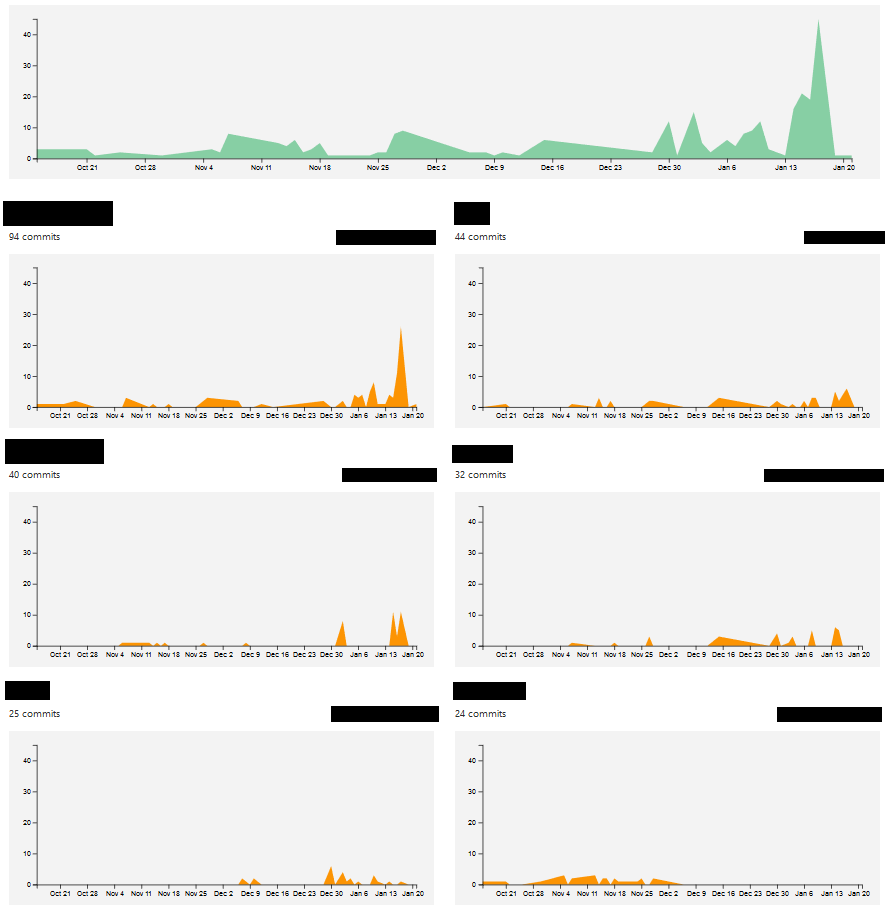
\includegraphics[scale=0.4]{slike/aktivnost.PNG} %veličina slike u odnosu na originalnu datoteku i pozicija slike
			\centering
			\caption{Primjer slike s potpisom}
			\label{fig:promjene}
		\end{figure}
		
		\begin{figure}[H]
			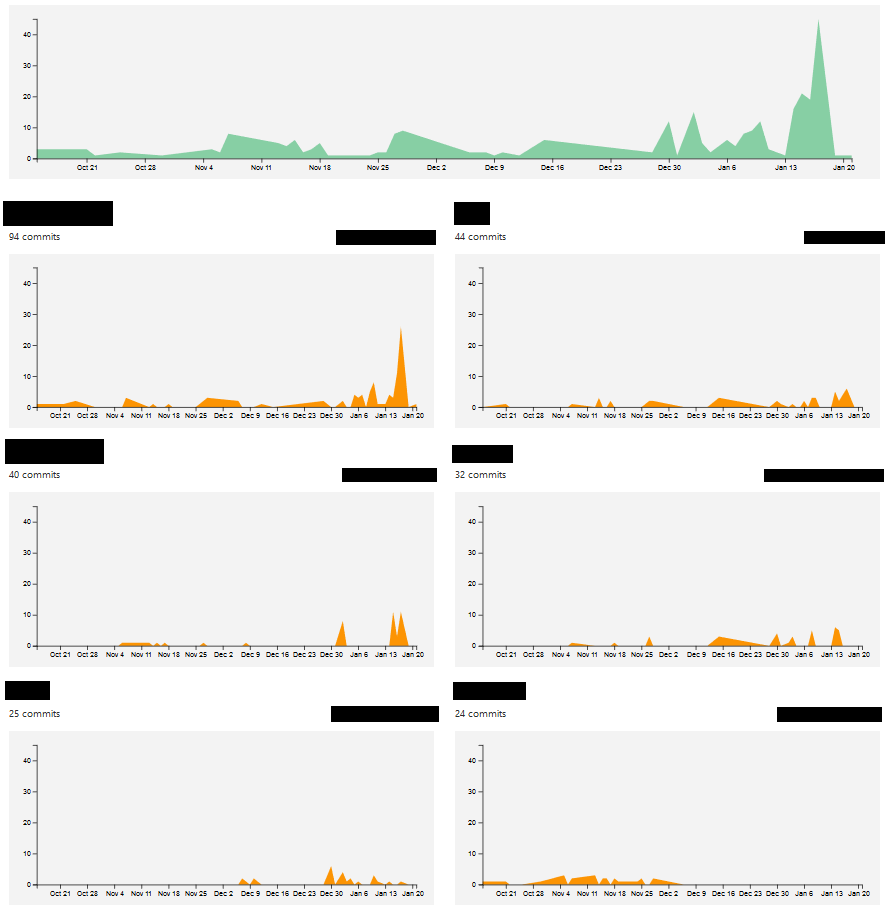
\includegraphics[width=\textwidth]{slike/aktivnost.PNG} %veličina u odnosu na širinu linije
			\caption{Primjer slike s potpisom 2}
			\label{fig:promjene2} %label mora biti drugaciji za svaku sliku
		\end{figure}
		
		Referenciranje slike \ref{fig:promjene2} u tekstu.
		
		\eject
		
	
	\chapter{Specifikacija programske potpore}
		
	\section{Funkcionalni zahtjevi}


			\noindent \textbf{Dionici:}
			
			\begin{packed_enum}
				
				\item Primarni dionici:
				
				\begin{packed_enum}
					\item Naručitelj
					\item Razvojni tim
					\item Rukovoditelji razvoja
					\item Strateški klijenti
					\item Superadministrator
					\item Administrator
				\end{packed_enum}
				
				\item Sekundarni dionici:	
				
				\begin{packed_enum}
					\item Sudionici konferencije
					\item Zaposlenici konferencije
					\item Autori	
				\end{packed_enum}		
				
			\end{packed_enum}
			
			\noindent \textbf{Akteri i njihovi funkcionalni zahtjevi:}
			
			
			\begin{packed_enum}
				\item Neregistrirani posjetitelji konferencije
				
			\begin{quote}
				Neregistrirani posjetitelji konferencije imaju mogućnost pregledavanja stručnih postera svih prijavljenih sudionika pomoću lozinke dobivene na konferenciji i imaju mogućnost dodatne registracije u sustav po želji.
			\end{quote}
				
				\item Registrirani posjetitelji konferencije
				
		\begin{quote}
			Registrirani posjetitelji konferencije imaju dodatnu mogućnost glasanja za stručni poster za koji smatraju da je najbolji i pristup rezultatima glasovanja kako bi vidjeli koji su posteri osvojili najviše glasova. Također mogu pratiti trenutna događanja u glavnoj konferencijskoj dvorani putem direktnog videoprijenosa. Nadalje, imaju priliku vidjeti promotivne materijale pokrovitelja konferencije te podatke o trenutnim vremenskim uvjetima i vremenskoj prognozi za navedenu lokaciju. Za vrijeme trajanja konferencije registrirani posjetitelji moći će pregledavati i preuzimati objavljene fotografije s konferencije.
		\end{quote}
		
				\item Superadministrator
				\begin{quote}
					Superadministrator ima mogućnost davanja administratorskih uloga već postojećim računima.
				\end{quote}
				
				\item Administrator
				\begin{quote}
					Administrator ima mogućnost kreiranja nove konferencije. Prilikom kreiranja konferencije, administrator može odabrati njezin naziv, opis konferencije, mjesto održavanja, njezin početak kao i njezin kraj. Inicijalnu lozinku konferencije sustav automatski generira.
				\end{quote}
				
				\item Autori
				\begin{quote}
					Autori su glavni sudionici konferencije koji će prezentirati svoje radove. Oni prije početka konferencije elektroničkom poštom dostavljaju sve potrebne materijale (postere) sistemskom administratoru. Također, nakon završetka konferencije elektroničkom poštom dobivaju informaciju o rangu njihovih radova kao i pozivnicu za dodjelu nagrada.
				\end{quote}
				
				\item Pokrovitelji
				\begin{quote}
					Pokrovitelji financiraju samu konferenciju i dostavljaju promotivne materijale sistemskom administratoru koji će omogućiti njihov prikaz registriranim posjetiteljima.
				\end{quote}
				
				
				\item Aplikacija i baza podataka
				\begin{quote}
					Pasivni faktori same funkcionalnosti aplikacije kao i spremanja podataka.
				\end{quote}
			\end{packed_enum}
			
			\eject 
			
			
				
			\subsection{Obrasci uporabe}
									
					\noindent \underbar{\textbf{UC1 - Prijava u sustav odgovarajućom lozinkom}}
					\begin{packed_item}
						
						\item \textbf{Glavni sudionik: } Svi posjetitelji konferencije
						\item  \textbf{Cilj:} Prijava u sustav
						\item  \textbf{Sudionici:} Aplikacija i baza podataka
						\item  \textbf{Preduvjet:} Odgovarajuća lozinka dostupna svim posjetiteljima konferencije
						\item  \textbf{Opis osnovnog tijeka:}
						
						\item[] \begin{packed_enum}
							
							\item Posjetitelj upisuje lozinku dobivenu na konferenciji 
							\item Sustav provjerava odgovara li kriptografski sažetak lozinke upisane od strane korisnika onoj u bazi podataka
							\item Ukoliko je lozinka točna, posjetitelj se uspješno prijavljuje u aplikaciju
							\item Prijavljenom korisniku otvara se nova stranica
						\end{packed_enum}
						
						\item  \textbf{Opis mogućih odstupanja:}
						
						\item[] \begin{packed_item}
							
							\item[1.a] Posjetitelj je upisao pogrešnu lozinku
							\item[] \begin{packed_enum}
								
								\item Posjetitelj dobiva obavijest od strane aplikacije kako je njegova lozinka neispravna
								\item Od posjetitelja se traži da opet upiše lozinku
								
							\end{packed_enum}
						
							
						\end{packed_item}
					\end{packed_item}
					
					\noindent \underbar{\textbf{UC2 - Odjava prijavljenog korisnika}}
					\begin{packed_item}
						
						\item \textbf{Glavni sudionik: }Korisnik
						\item  \textbf{Cilj:} Odjava prijavljenog korisnika
						\item  \textbf{Sudionici:} Aplikacija i baza podataka
						\item  \textbf{Preduvjet:} Korisnik je prijavljen u sustav
						\item  \textbf{Opis osnovnog tijeka:}
						
						\item[] \begin{packed_enum}
							
							\item Posjetitelj se uspješno prijavio u sustav odgovarajućom lozinkom
							\item Korisnik je pritisnuo gumb za odjavu prijavljenih korisnika iz sustava 
							\item Sustav ga uspješno odjavljuje i vraća na početnu stranicu
							
						\end{packed_enum}
						
						\item  \textbf{Opis mogućih odstupanja:}
						
						\item[] \begin{packed_item}
							
							\item[1.a] Korisnik se nije uspješno prijavio u sustav
							\item[] \begin{packed_enum}
								
								\item Od strane korisnika zahtijeva se da se prijavi u sustav odgovarajućom lozinkom
								
							\end{packed_enum}
							
							
						\end{packed_item}
					\end{packed_item}
					
					
					\noindent \underbar{\textbf{UC3 - Pregledavanje stručnih postera prijavljenih korisnika}}
					\begin{packed_item}
						
						\item \textbf{Glavni sudionik: }Korisnik
						\item  \textbf{Cilj:} Pregledavanje stručnih postera
						\item  \textbf{Sudionici:} Aplikacija i baza podataka
						\item  \textbf{Preduvjet:} Korisnik je prijavljen u sustav
						\item  \textbf{Opis osnovnog tijeka:}
						
						\item[] \begin{packed_enum}
							
							\item Aplikacija dohvaća potrebne materijale i postere iz baze podataka
							\item Korisnik ima mogućnost pregledavanja stručnih postera
							
						\end{packed_enum}
						
					\end{packed_item}
					
				
				
				
				\noindent \underbar{\textbf{UC4 - Registracija u sustav prijavljenih korisnika}}
				\begin{packed_item}
					
					\item \textbf{Glavni sudionik: }Korisnik
					\item  \textbf{Cilj:} Registracija u sustav već prijavljenih korisnika
					\item  \textbf{Sudionici:} Aplikacija i baza podataka
					\item  \textbf{Preduvjet:} Korisnik je prijavljen u sustav
					\item  \textbf{Opis osnovnog tijeka:}
					
					\item[] \begin{packed_enum}
						
						\item Korisnik je pritisnuo gumb za registraciju u sustav
						\item Korisniku se otvara nova stranica s poljem za upis adrese elektroničke pošte i nove lozinke
						\item Sustav provjerava valjanost upisane adrese elektroničke pošte kao i lozinke
						\item Adresa elektroničke pošte registriranog korisnika sprema se u bazu podataka dok se upisana lozinka kriptira te se njezin sažetak sprema u bazu 

					\end{packed_enum}
					
					\item  \textbf{Opis mogućih odstupanja:}
					
					\item[] \begin{packed_item}
						
						\item[3.a] Pogrešan unos elektroničke pošte
						\item[] \begin{packed_enum}
							
							\item Sustav provjerava ispravnost formata unesene adrese elektroničke pošte te ukoliko je kriva, obavještava korisnika o traženom formatu
							\item Korisnik upisuje ispravan format adrese elektroničke pošte
							
						\end{packed_enum}
						\item[3.b] Pogrešan unos lozinke
						\item[] \begin{packed_enum}
							
							\item Sustav provjerava ispravnost formata unesene lozinke te ukoliko je kriva, obavještava korisnika o traženom formatu
							\item Korisnik upisuje ispravan format lozinke
							
						\end{packed_enum}
						
						\item[4.a] Korisnik je već prijavljen u sustav
						\item[] \begin{packed_enum}
							
							\item Sustav provjerava postoji li već registriran korisnik s istom adresom elektroničke pošte
							\item Sustav odbija registraciju korisnika te ga obavještava kako je korisnik već registriran 
							
						\end{packed_enum}
						
					\end{packed_item}
				\end{packed_item}
				
				
				
				\noindent \underbar{\textbf{UC5 - Odjava registriranog korisnika}}
				\begin{packed_item}
					
					\item \textbf{Glavni sudionik: }Korisnik
					\item  \textbf{Cilj:} Odjava iz sustava registriranog korisnika
					\item  \textbf{Sudionici:} Aplikacija i baza podataka
					\item  \textbf{Preduvjet:} Registrirani korisnik prijavljen je u sustav
					\item  \textbf{Opis osnovnog tijeka:}
					
					\item[] \begin{packed_enum}
						
						\item Korisnik je pritisnuo gumb za odjavu registriranih korisnika iz sustava 
						\item Sustav ga uspješno odjavljuje i vraća na početnu stranicu prijavljenih korisnika
						
					\end{packed_enum}
					
				\end{packed_item}
				
				
				\noindent \underbar{\textbf{UC6 - Glasanje za najbolji stručni poster konferencije}}
				\begin{packed_item}
					
					\item \textbf{Glavni sudionik: }Korisnik
					\item  \textbf{Cilj:} Glasanje za najbolji stručni poster konferencije
					\item  \textbf{Sudionici:} Aplikacija i baza podataka
					\item  \textbf{Preduvjet:} Glasovanje je moguće samo registriranim korisnicima tijekom određenog vremenskog razdoblja koje je određeno danima i vremenom održavanja konferencije
					\item  \textbf{Opis osnovnog tijeka:}
					
					\item[] \begin{packed_enum}
						
						\item Registrirani korisnik pregledava objavljene stručne postere
						\item Nakon što registrirani korisnik odabere njemu najbolji poster, ima mogućnost glasanja za taj poster
						\item Registrirani korisnik pritišće gumb za glasanje za određeni poster
						\item Aplikacija sprema u bazu podataka taj glas i označava da je taj korisnik glasao i da više nema mogućnost glasanja

					\end{packed_enum}
					
					\item  \textbf{Opis mogućih odstupanja:}
					
					\item[] \begin{packed_item}
						
						\item[3.a] Registrirani korisnik pritišće gumb za glasanje za određeni poster van vremenskog razdoblja predviđenog za glasanje
						\item[] \begin{packed_enum}
							
							\item Registrirani korisnik pritišće gumb za glasanje za određeni poster
							\item Sustav ga obavještava kako ne može glasati budući da glasovanje još nije započeto te mu javlja točno vrijeme početka glasanja ili da je glasovanje završilo
							
						\end{packed_enum}
						
						\item[3.b] Registrirani korisnik pritišće gumb za glasanje za drugi poster
						\item[] \begin{packed_enum}
							
							\item Registrirani korisnik pritišće gumb za glasanje za poster nakon što je već jednom glasao za neki drugi poster
							\item Sustav ga obavještava kako ne može glasati budući da je već jednom glasao
							
						\end{packed_enum}
						
						
					\end{packed_item}
				\end{packed_item}
				
				
				\noindent \underbar{\textbf{UC7 - Povlačenje korisnikovog glasa stručnog postera}}
				\begin{packed_item}
					
					\item \textbf{Glavni sudionik: }Korisnik
					\item  \textbf{Cilj:} Povlačenje korisnikovog glasa za stručni poster
					\item  \textbf{Sudionici:} Aplikacija i baza podataka
					\item  \textbf{Preduvjet:} Povlačenje glasa moguće je samo registriranim korisnicima koji su već glasali tijekom određenog vremenskog razdoblja koje je određeno danima i vremenom održavanja konferencije
					\item  \textbf{Opis osnovnog tijeka:}
					
					\item[] \begin{packed_enum}
						
						\item Korisnik je odlučio promijeniti svoje mišljenje te želi povući svoj glas za već odabrani stručni poster
						\item Registrirani korisnik pritišće gumb za povlačenje glasa za određeni poster
						\item Aplikacija briše iz baze podataka taj glas i označava da taj korisnik može ponovno glasati
					\end{packed_enum}
					
					
				\end{packed_item}
				
				
				\noindent \underbar{\textbf{UC8 - Gledanje direktnog videoprijenosa konferencije}}
				\begin{packed_item}
					
					\item \textbf{Glavni sudionik: }Korisnik
					\item  \textbf{Cilj:} Gledanje direktnog videoprijenosa konferencije
					\item  \textbf{Sudionici:} Aplikacija i baza podataka
					\item  \textbf{Preduvjet:} Gledanje direktnog videoprijenosa konferencije moguće je samo registriranim korisnicima tijekom određenog vremenskog razdoblja koje je određeno danima i vremenom održavanja konferencije
					\item  \textbf{Opis osnovnog tijeka:}
					
					\item[] \begin{packed_enum}
						
						\item Registrirani korisnik pritišće gumb za direktno praćenje videoprijenosa konferencije 
						\item Aplikacija dohvaća iz baze podataka potreban videoprijenos te se korisniku prikazuje videoprozor
					\end{packed_enum}
					
					\item  \textbf{Opis mogućih odstupanja:}
					
					\item[] \begin{packed_item}
						
						\item[1.a] Registrirani korisnik pritišće gumb za direktno praćenje videoprijenosa konferencije van vremenskog razdoblja predviđenog za direktni videoprijenos konferencije
						\item[] \begin{packed_enum}
							
							\item Registrirani korisnik pritišće gumb za direktno praćenje videoprijenosa konferencije 
							\item Sustav ga obavještava kako ne može gledati direktan videoprijenos konferencije budući da on još nije započeo te mu javlja točno vrijeme početka konferencije
							
						\end{packed_enum}
				
						
					\end{packed_item}
				\end{packed_item}
				
				
				
				\noindent \underbar{\textbf{UC9 - Zatvaranje direktnog videoprijenosa konferencije}}
				\begin{packed_item}
					
					\item \textbf{Glavni sudionik: }Korisnik
					\item  \textbf{Cilj:} Zatvaranje direktnog videoprijenosa konferencije
					\item  \textbf{Sudionici:} Aplikacija i baza podataka
					\item  \textbf{Preduvjet:} Zatvaranje direktnog videoprijenosa konferencije moguće je samo registriranim korisnicima koji gledaju direktan videoprijenos konferencije tijekom određenog vremenskog razdoblja koje je određeno danima i vremenom održavanja konferencije
					\item  \textbf{Opis osnovnog tijeka:}
					
					\item[] \begin{packed_enum}
						
						\item Registrirani korisnik pritišće gumb za zatvaranje direktnog videoprijenosa konferencije 
						\item Aplikacija zatvara videoprozor
						
						
					\end{packed_enum}
					
				\end{packed_item}
				
				
				\noindent \underbar{\textbf{UC10 - Pregled poretka stručnih postera}}
				\begin{packed_item}
					
					\item \textbf{Glavni sudionik: }Korisnik
					\item  \textbf{Cilj:} Pregled poretka stručnih postera
					\item  \textbf{Sudionici:} Aplikacija i baza podataka
					\item  \textbf{Preduvjet:} Pregled poretka stručnih postera dostupan je svim registriranim korisnicima po završetku konferencije i glasanja
					\item  \textbf{Opis osnovnog tijeka:}
					
					\item[] \begin{packed_enum}
						
						\item Konferencija je kao i njeno glasanje završila
						\item Aplikacija iz baze podataka dohvaća glasove za stručne postere te prikazuje poredak najboljih stručnih postera svim registriranim korisnicima 
					\end{packed_enum}
					
					\item  \textbf{Opis mogućih odstupanja:}
					
					\item[] \begin{packed_item}
						
						\item[2.a] Poredak nije dostupan
						\item[] \begin{packed_enum}
							
							\item Prostor za poredak stručnih postera jest prazan
							\item Glasanje kao i sama konferencija nisu još završeni te sustav obavještava korisnika o vremenu objave poretka
							
						\end{packed_enum}
				
						
					\end{packed_item}
				\end{packed_item}
				
				
				
				\noindent \underbar{\textbf{UC11 - Gledanje promotivnih materijala pokrovitelja}}
				\begin{packed_item}
					
					\item \textbf{Glavni sudionik: }Korisnik
					\item  \textbf{Cilj:} Gledanje promotivnih materijala pokrovitelja
					\item  \textbf{Sudionici:} Aplikacija i baza podataka
					\item  \textbf{Preduvjet:} Mogućnost gledanja promotivnih materijala pokrovitelja imaju registrirani korisnici
					\item  \textbf{Opis osnovnog tijeka:}
					
					\item[] \begin{packed_enum}
						\item Aplikacija iz baze podataka dohvaća promotivne materijale pokrovitelja konferencije
						\item Na početnoj stranici dostupni su promotivni materijali pokrovitelja koje registrirani korisnik može gledati
					\end{packed_enum}
					
				\end{packed_item}
				
					\noindent \underbar{\textbf{UC12 - Prikaz dodatnih informacija konferencije kao što su vremenski uvjeti i lokacija}}
				\begin{packed_item}
					
					\item \textbf{Glavni sudionik: }Korisnik
					\item  \textbf{Cilj:} Prikaz dodatnih informacija konferencije kao što su vremenski uvjeti i lokacija
					\item  \textbf{Sudionici:} Aplikacija i baza podataka
					\item  \textbf{Preduvjet:} Korisnik mora biti registriran u sustav
					\item  \textbf{Opis osnovnog tijeka:}
					
					\item[] \begin{packed_enum}
						
						\item Aplikacija iz baze podataka dohvaća dodatne podatke o konferenciji kao što su vremenski uvjeti i lokacija
						\item Na početnoj stranici dostupne su dodatne informacije o konferenciji kao što su vremenski uvjeti i lokacija koje registrirani korisnik može gledati
					\end{packed_enum}
					
				\end{packed_item}
				
				
					\noindent \underbar{\textbf{UC13 - Prikaz objavljenih fotografija s konferencije}}
				\begin{packed_item}
					
					\item \textbf{Glavni sudionik: }Korisnik
					\item  \textbf{Cilj:} Prikaz objavljenih fotografija
					\item  \textbf{Sudionici:} Aplikacija i baza podataka
					\item  \textbf{Preduvjet:} Korisnik mora biti registriran u sustav te su fotografije vidljive samo za vrijeme trajanja konferencije
					\item  \textbf{Opis osnovnog tijeka:}
					
					\item[] \begin{packed_enum}
						
						\item Aplikacija iz baze podataka dohvaća odabrane fotografije s konferencije
						\item Na početnoj stranici dostupne su odabrane fotografije s konferencije 
						
					\end{packed_enum}
					
					\item  \textbf{Opis mogućih odstupanja:}
					
					\item[] \begin{packed_item}
						
						\item[2.a] Korisnik ne vidi fotografije
						\item[] \begin{packed_enum}
							
							\item Korisnik na početnoj stranici ne vidi fotografije s konferencije
							\item Sustav obavještava korisnika kako fotografije s konferencije nisu dostupne budući da je konferencija završena 
							
						\end{packed_enum}
						
					\end{packed_item}
				\end{packed_item}
				
				
				\noindent \underbar{\textbf{UC14 - Preuzimanje objavljenih fotografija s konferencije}}
				\begin{packed_item}
					
					\item \textbf{Glavni sudionik: }Korisnik
					\item  \textbf{Cilj:} Preuzimanje objavljenih fotografija s konferencije
					\item  \textbf{Sudionici:} Aplikacija i baza podataka
					\item  \textbf{Preduvjet:} Korisnik mora biti registriran u sustav te su fotografije dostupne za preuzimanje samo za vrijeme trajanja konferencije
					\item  \textbf{Opis osnovnog tijeka:}
					
					\item[] \begin{packed_enum}
						
						\item Aplikacija iz baze podataka dohvaća odabrane fotografije s konferencije
						\item Korisnik pritišće gumb za preuzimanje fotografije na svoj uređaj
						
					\end{packed_enum}
					
				\end{packed_item}
				
				\noindent \underbar{\textbf{UC15 - Dodavanje autora i njihovih stručnih postera u bazu podataka}}
				\begin{packed_item}
					
					\item \textbf{Glavni sudionik: } Administrator
					\item  \textbf{Cilj:} Dodavanje autora i njihovih stručnih postera u bazu podataka
					\item  \textbf{Sudionici:} Baza podataka i aplikacija
					\item  \textbf{Preduvjet:} Administratoru su dostavljeni svi potrebni materijali za dodavanje autora kao i njihovih stručnih postera
					\item  \textbf{Opis osnovnog tijeka:}
					
					\item[] \begin{packed_enum}
						
						\item Autor elektroničkom poštom šalje administratoru svoje podatke i stručni poster
						\item Administrator provjera valjanost podataka
						\item Ukoliko su svi podaci ispravni i valjani, administrator otvara sučelje za dodavanje autora i njegovog postera gdje upisuje sve potrebne informacije vezane za autora i poster te prilaže sam poster
						\item Nakon pritiska na gumb za spremanje, baza podataka sprema informacije o posteru kao i o njegovom autoru
						
					
					\end{packed_enum}
				\end{packed_item}
				
				
				\noindent \underbar{\textbf{UC16 - Definiranje svih potrebnih parametara za rad sustava}}
				\begin{packed_item}
					
					\item \textbf{Glavni sudionik: }Sistemski administrator
					\item  \textbf{Cilj:} Definiranje svih potrebnih parametara za rad sustava kao što su vrijeme početka i završetka konferencije, otvaranje i zatvaranje glasanja...
					\item  \textbf{Sudionici:} Baza podataka
					\item  \textbf{Preduvjet:} Sistemskom administratoru dostupne su sve potrebne informacije o konferenciji
					\item  \textbf{Opis osnovnog tijeka:}
					
					\item[] \begin{packed_enum}
						
						\item Sistemski administrator dobiva sve potrebne informacije o konferenciji
						\item Dobivene informacije sistemski administrator pohranjuje u bazu podataka
					\end{packed_enum}
					
				\end{packed_item}
				
				\noindent \underbar{\textbf{UC17 - Obavještavanje autora o njihovom uspjehu i mjestu održavanja dodjele nagrada}}
				\begin{packed_item}
					
					\item \textbf{Glavni sudionik: }Aplikacija 
					\item  \textbf{Cilj:} Obavještavanje autora o njihovom uspjehu i mjestu održavanja dodjele nagrada
					\item  \textbf{Sudionici:} Autori
					\item  \textbf{Preduvjet:} Glasanje je kao i sama konferencija završeno
					\item  \textbf{Opis osnovnog tijeka:}
					
					\item[] \begin{packed_enum}
						
						\item Aplikacija iz baze podataka dohvaća podatke o poretku radova
						\item Autori prva tri najbolja rada dobivaju posebnu čestitku i pozivnicu za dodjelu nagrade dok ostali autori dobivaju samo pozivnicu za dolazak na dodjelu nagrada
					\end{packed_enum}
					
				\end{packed_item}	
				
				
				\noindent \underbar{\textbf{UC18 - Dodavanje administratorske uloge postojećim registriranim korisnicima}}
				\begin{packed_item}
					
					\item \textbf{Glavni sudionik: } Superadministrator
					\item  \textbf{Cilj:} Dodavanje administratorske uloge postojećim registriranim korisnicima
					\item  \textbf{Sudionici:} Registrirani korisnici, baza podataka
					\item  \textbf{Preduvjet:} Korisnik se mora registrirati
					\item  \textbf{Opis osnovnog tijeka:}
					
					\item[] \begin{packed_enum}
						
						\item Nakon prijavljivanja u sustav superadministratoru se otvara lista svih već postojećih administratora
						\item Superadministrator po želji može kreirati novog administratora 
					\end{packed_enum}
					
					\item  \textbf{Opis mogućih odstupanja:}
					
					\item[] \begin{packed_item}
						
						\item[1.a] Superadministrator ne vidi niti jednog administratora
						\item[] \begin{packed_enum}
							
							\item U bazi podataka nema niti jednog administratora
							\item Superadministrator mora kreirati barem jednog administratora da bi mu se pojavila lista 
							
						\end{packed_enum}
						
					\end{packed_item}
				\end{packed_item}
				
				\noindent \underbar{\textbf{UC19 - Kreiranje konferencije}}
				\begin{packed_item}
					
					\item \textbf{Glavni sudionik: } Administrator
					\item  \textbf{Cilj:} Kreiranje konferencije
					\item  \textbf{Sudionici:} Aplikacija i baza podataka
					\item  \textbf{Preduvjet:} Korisnik mora imati ulogu administratora
					\item  \textbf{Opis osnovnog tijeka:}
					
					\item[] \begin{packed_enum}
						
						\item Nakon prijave u sustav administrator ima mogućnost kreiranja nove konferencije
						\item Administratoru se otvara sučelje za kreiranje nove konferencije s praznim poljima za naziv konferencije, opis konferencije, mjesto održavanja, datum početka kao i datum završetka konferencije koje administrator može popuniti po želji
						\item Nakon popunjavanja sustav će automatski generirati inicijalnu lozinku konferencije te će se čitava konferencija spremiti u bazu podataka
					\end{packed_enum}
	
					
					
				\end{packed_item}
				
			
				
				\noindent \underbar{\textbf{UC20 - Dodavanje fotografija za konferenciju}}
				\begin{packed_item}
					
					\item \textbf{Glavni sudionik: } Administrator
					\item  \textbf{Cilj:} Dodavanje fotografija za konferenciju
					\item  \textbf{Sudionici:} Aplikacija i baza podataka
					\item  \textbf{Preduvjet:} Korisnik mora imati ulogu administratora
					\item  \textbf{Opis osnovnog tijeka:}
					
					\item[] \begin{packed_enum}
						
						\item Nakon prijave u sustav administrator ima mogućnost dodavanja fotografija u bazu podataka
						\item Administrator otvara sučelje za dodavanje novih fotografija gdje upisuje potrebne informacije vezane za fotografije te prilaže fotografiju
						\item Nakon pritiska na gumb za spremanje, baza podatka sprema informacije o fotografiji
					\end{packed_enum}
					
					\item  \textbf{Opis mogućih odstupanja:}
					
					\item[] \begin{packed_item}
						
						\item[2.a] Unos krivih podataka
						\item[] \begin{packed_enum}
							
							\item Administrator je unio neke krive podatke
							\item Sustav ga upozorava na krive podatke te mu javlja kako da ispravi pogrešku
							
						\end{packed_enum}
						
						
					\end{packed_item}
				\end{packed_item}
				
				\noindent \underbar{\textbf{UC21 - Dodavanje promotivnih materijala za konferenciju}}
				\begin{packed_item}
					
					\item \textbf{Glavni sudionik: } Administrator
					\item  \textbf{Cilj:} Dodavanje promotivnih materijala za konferenciju
					\item  \textbf{Sudionici:} Aplikacija i baza podataka
					\item  \textbf{Preduvjet:} Korisnik mora imati ulogu administratora
					\item  \textbf{Opis osnovnog tijeka:}
					
					\item[] \begin{packed_enum}
						
						\item Nakon prijave u sustav administrator ima mogućnost dodavanja promotivnih materijala u bazu podataka
						\item Administrator otvara sučelje za dodavanje novih promotivnih materijala gdje upisuje potrebne informacije vezane za promotivne materijale te prilaže promotivni materijal
						\item Nakon pritiska na gumb za spremanje, baza podatka sprema informacije o promotivnom materijalu
					\end{packed_enum}
					
					\item  \textbf{Opis mogućih odstupanja:}
					
					\item[] \begin{packed_item}
						
						\item[2.a] Unos krivih podataka
						\item[] \begin{packed_enum}
							
							\item Administrator je unio neke krive podatke
							\item Sustav ga upozorava na krive podatke te mu javlja kako da ispravi pogrešku
							
						\end{packed_enum}
						
						
					\end{packed_item}
				\end{packed_item}
				
					
				\subsubsection{Dijagrami obrazaca uporabe}
				
					\begin{figure}[H]
						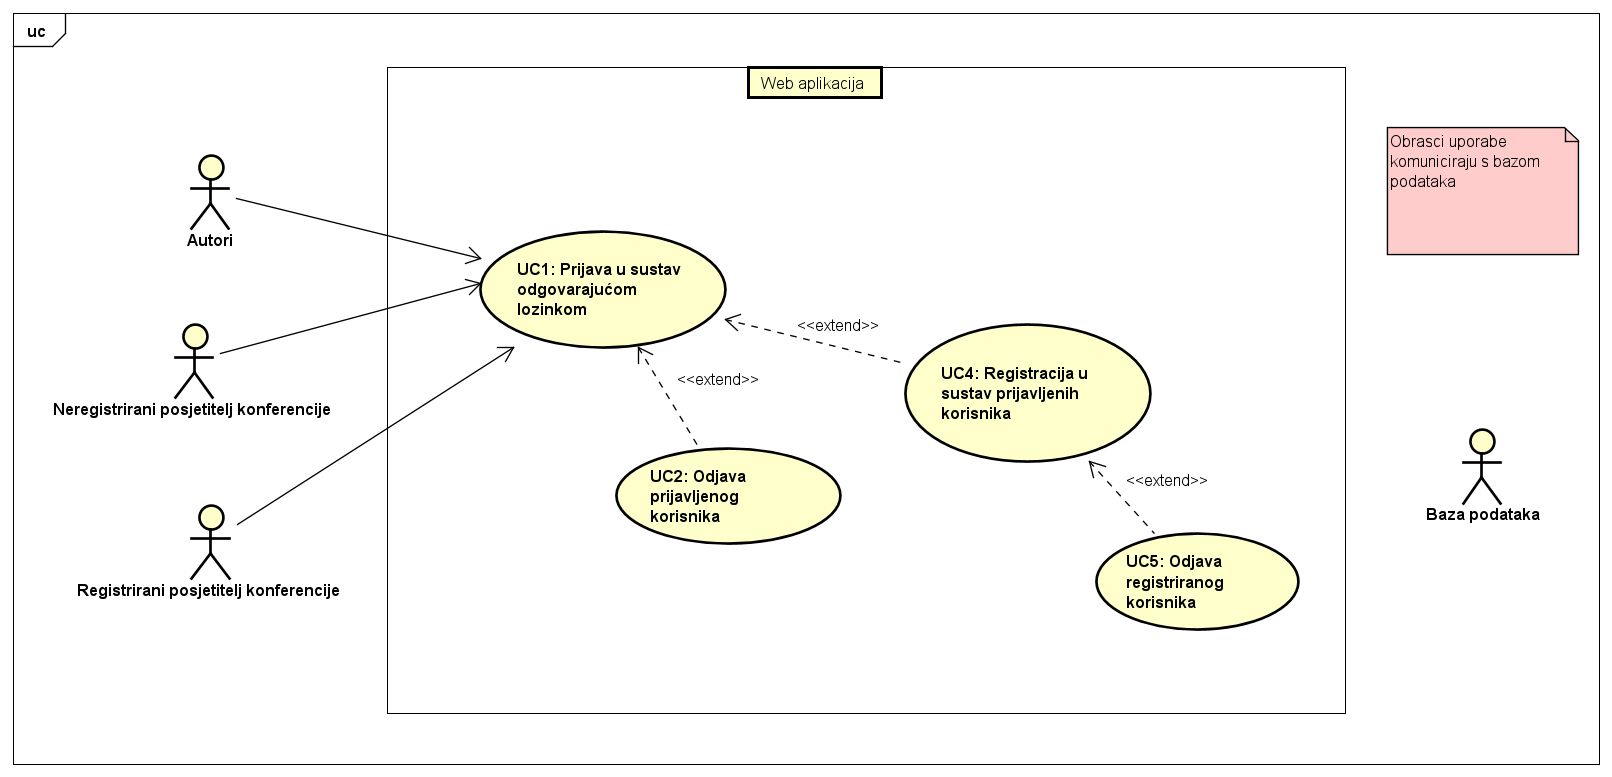
\includegraphics[width=\textwidth]{slike/prijavaUseCase.PNG} %veličina u odnosu na širinu linije
						\caption{Dijagram obrazaca uporabe, prijava u sustav}
						\label{fig:prijava-dijagram} %label mora biti drugaciji za svaku sliku
					\end{figure}
					
					\begin{figure}[H]
						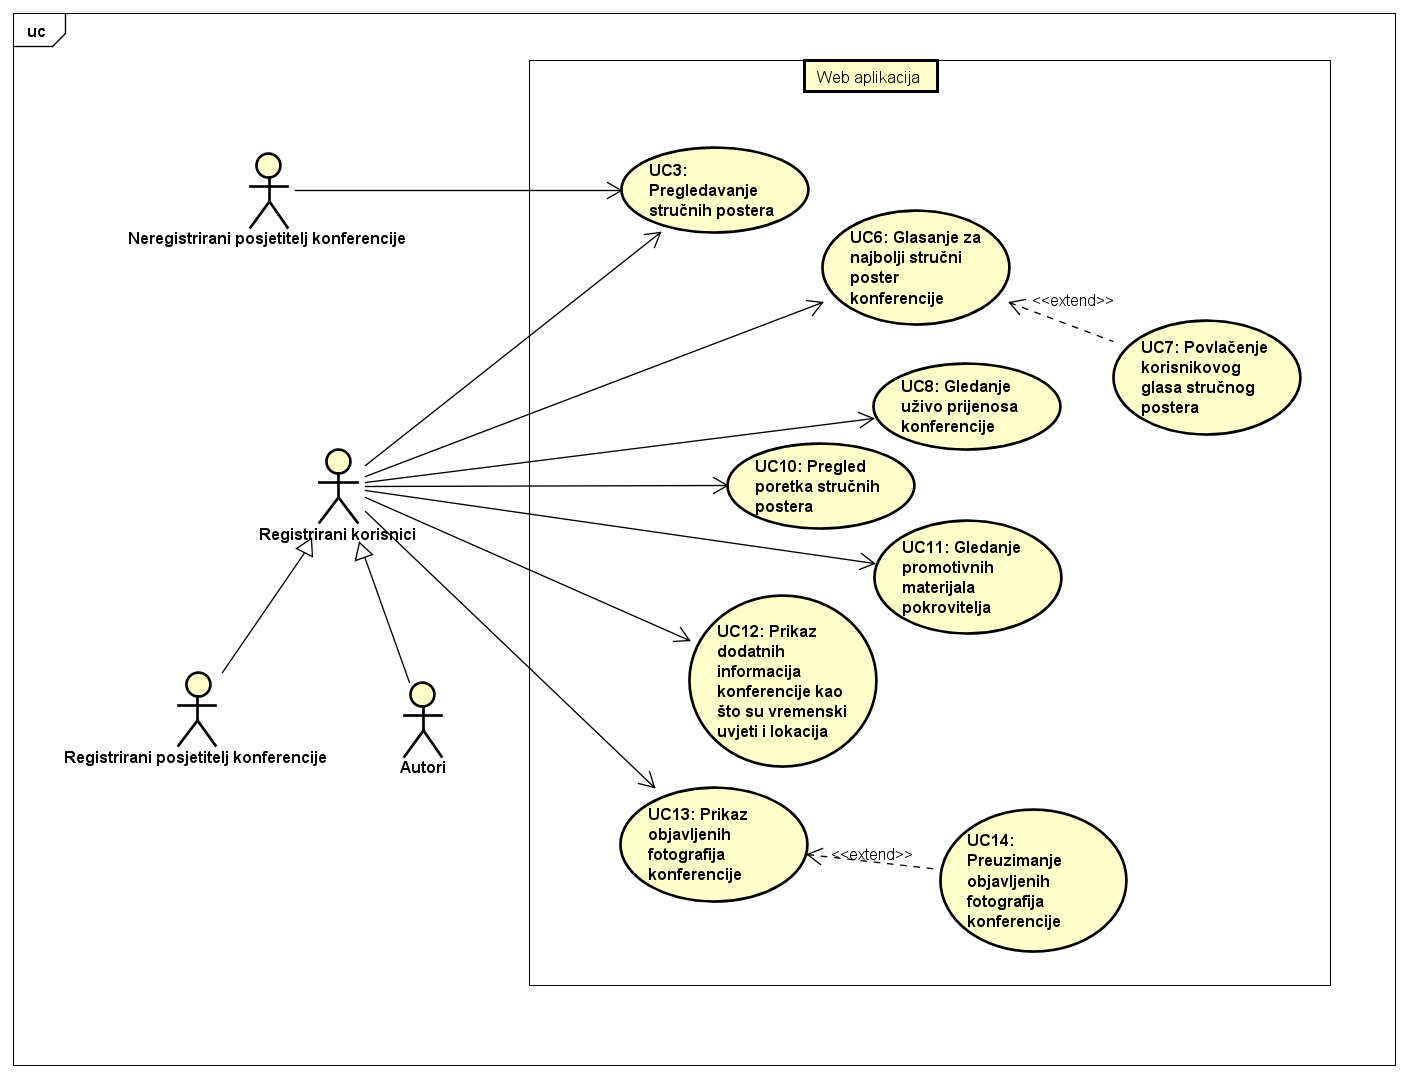
\includegraphics[width=\textwidth]{slike/korisniciUseCase.PNG} %veličina u odnosu na širinu linije
						\caption{Dijagram obrazaca uporabe, funkcionalnosti korisnika}
						\label{fig:korisnik-dijagram} %label mora biti drugaciji za svaku sliku
					\end{figure}
					
					\begin{figure}[H]
						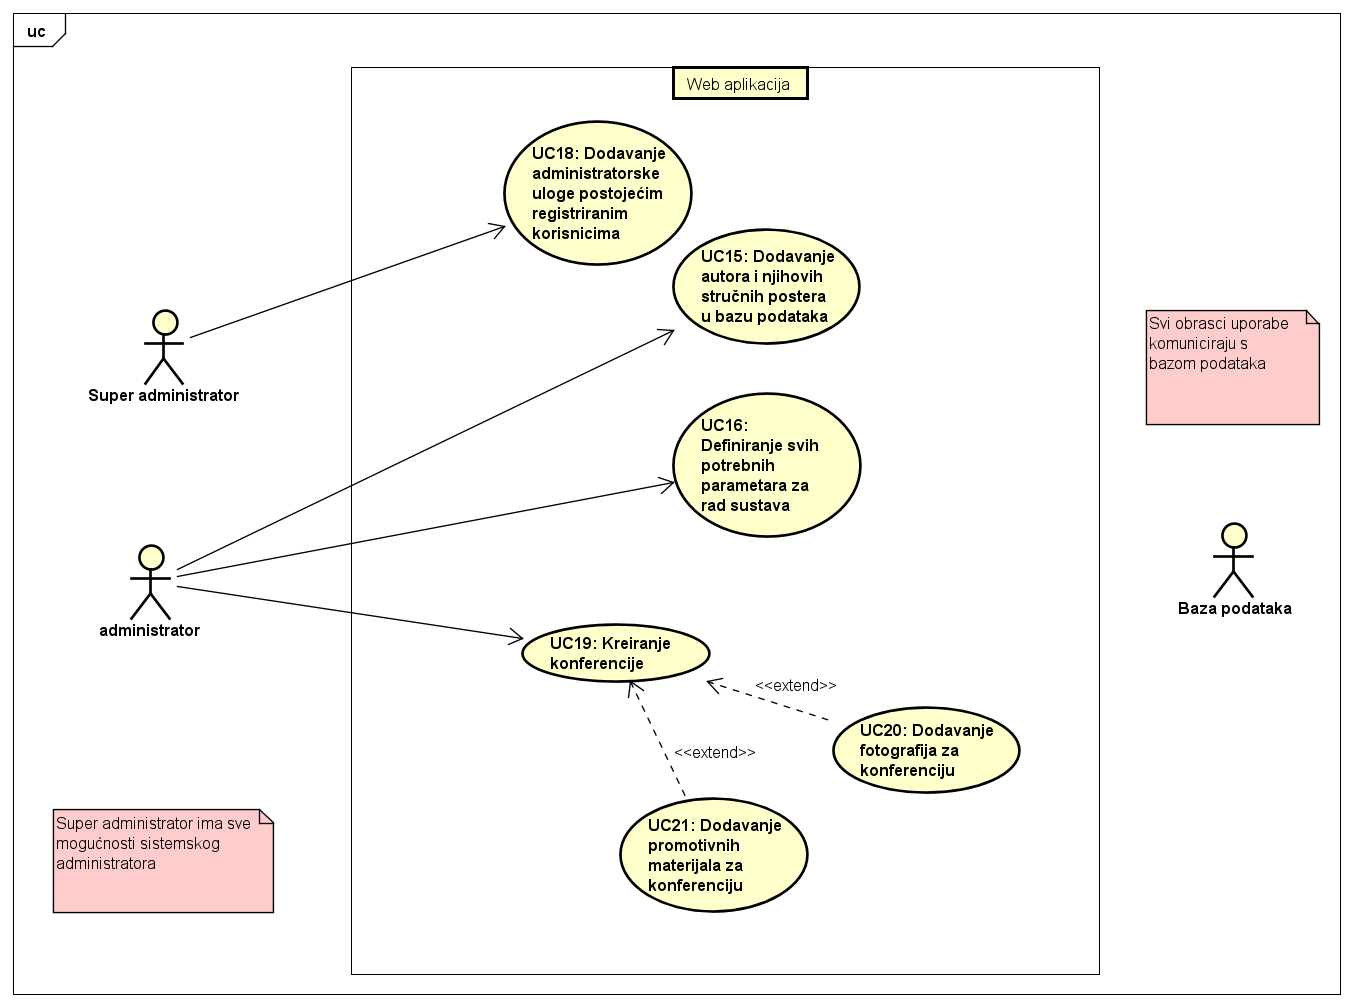
\includegraphics[width=\textwidth]{slike/adminUseCase.PNG} %veličina u odnosu na širinu linije
						\caption{Dijagram obrazaca uporabe, funkcionalnosti administratora}
						\label{fig:admin-dijagram} %label mora biti drugaciji za svaku sliku
					\end{figure}
					
				\eject		
				
			\subsection{Sekvencijski dijagrami}
						
				\textbf{Obrazac uporabe UC1: Prijava u sustav odgovarajućom lozinkom}\\
				Korisnik na početnom zaslonu upisuje lozinku konferencije te ju šalje poslužitelju. Poslužitelj šalje upit bazi podataka i provjerava je li lozinka ispravna, ako je neispravna ovaj se postupak ponavlja do upisa točne lozinke. Ako je unesena lozinka ispravna, korisniku se potvrđuje da je unio ispravnu lozinku te se od baze podataka zatražuju podaci o konferenciji i oni se šalju korisniku.
				
				\begin{figure}[H]
					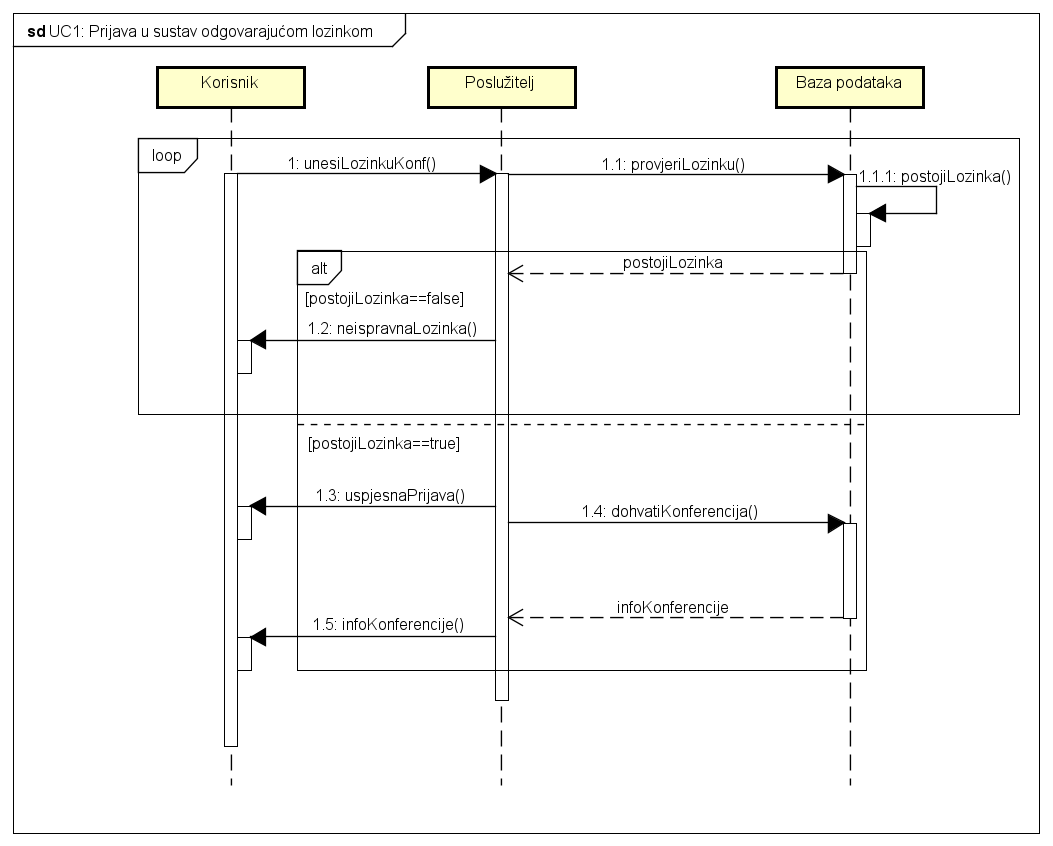
\includegraphics[width=\textwidth]{slike/uc1Sekvencijski.PNG} %veličina u odnosu na širinu linije
					\caption{Sekvencijski dijagram obrasca UC1: Prijava u sustav odgovarajućom lozinkom}
					\label{fig:uc1-sekvencijski} %label mora biti drugaciji za svaku sliku
				\end{figure}
				\eject
					\textbf{Obrazac uporabe UC4: Registracija u sustav prijavljenih korisnika}\\
				Korisnik klikom na gumb registracija pokreće postupak registracije. Sustav mu šalje nazad formu za registraciju u koju upisuje adresu elektroničke pošte i lozinku te ih šalje sustavu. Zatim sustav provjerava format adrese elektroničke pošte pa ako nije valjan obavještava korisnika o tome, inače nastavlja dalje i provjerava ispunjava li lozinka traženi format te u slučaju da ne ispunjava također obavještava korisnika. Na kraju se upitom nad bazom provjerava postoji li registrirani korisnik s tom adresom elektroničke pošte. U slučaju da postoji obavijestit ćemo korisnika o tome, a ako ne, lozinka će se kriptirati i spremiti zajedno s adresom elektroničke pošte u bazu podataka i korisnika ćemo obavijestiti da je registracija bila uspješna.
				
				\begin{figure}[H]
					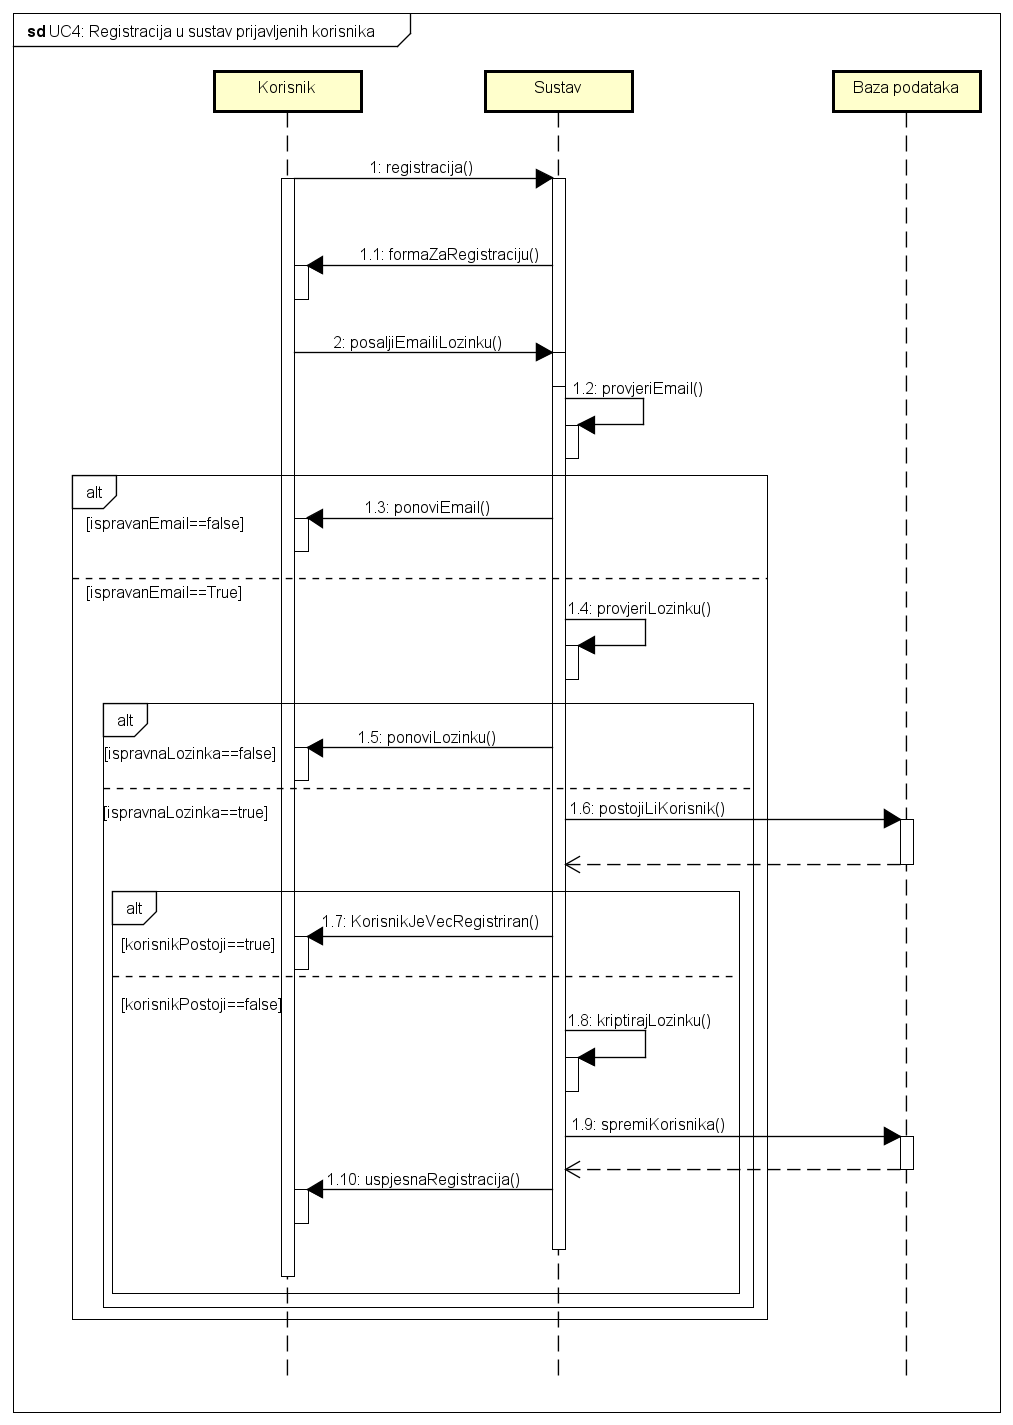
\includegraphics[width=\textwidth]{slike/uc4Sekvencijski.PNG} %veličina u odnosu na širinu linije
					\caption{Sekvencijski dijagram obrasca UC4: Registracija u sustav prijavljenih korisnika}
					\label{fig:uc4-sekvencijski} %label mora biti drugaciji za svaku sliku
				\end{figure}
				\eject
				
				\textbf{Obrazci uporabe UC6 i UC7: Glasanje}\\
				Obrasci UC6 i UC7 opisuju rad sustava glasovanja. Postupci glasanja i povlačenja glasa započinju zahtjevom korisnika, te se za oba prvo provjerava vremenski prozor glasanja (glasanje i promijena glasa je onemogućena ako je vremenski prozor glasanja prošao). Ako je glasanje još uvijek dozvoljeno sljedeći korak je provjera da li je korisnik već glasao, s obzirom na odgovor baze podataka imamo grananje. Kod UC6 ako je korisnik već glasao onda mu se javlja greška i nudi opcija da odmakne svoj glas, inače u bazu podataka se sprema glas, te se korisniko dojavljuje da je glasanje provedeno uspješno. Kod UC7 ako je korisnik već glasao, onda se glas uspješno briše iz baze podataka, inače se javlja korisniku greška da nije glasao prije.
				\begin{figure}[H]
					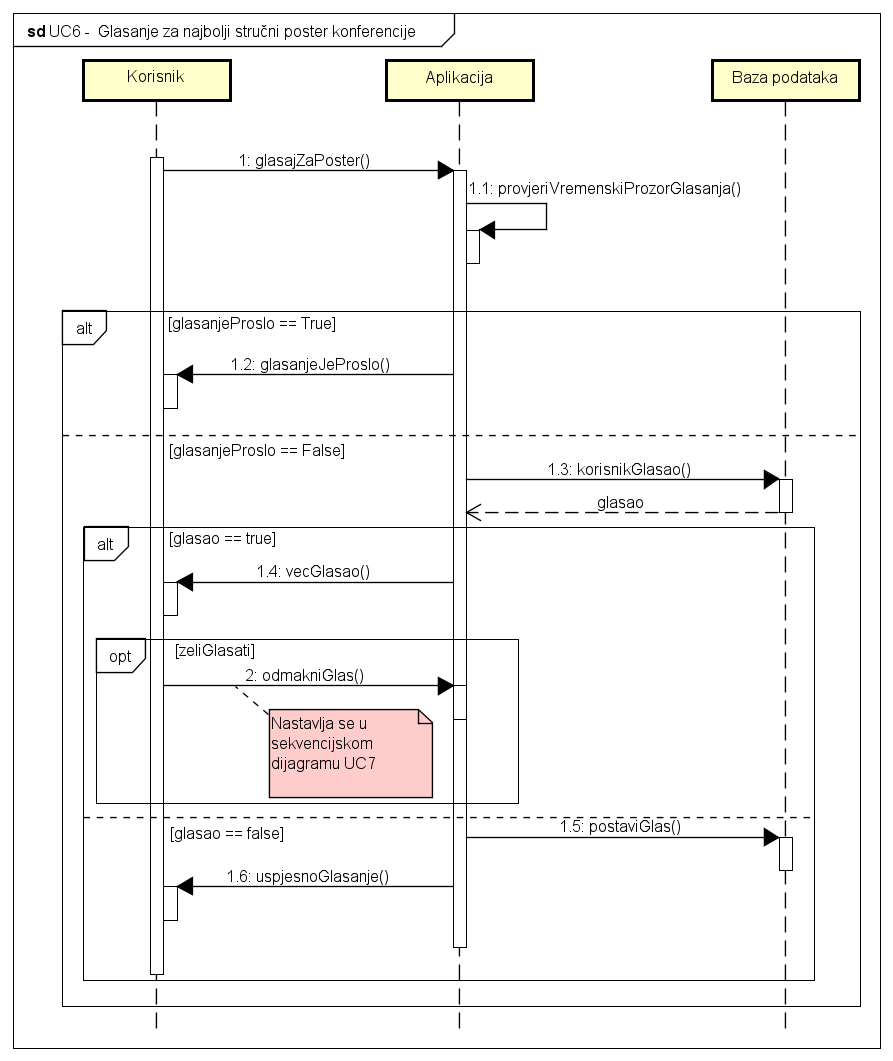
\includegraphics[width=\textwidth]{slike/uc6Sekvencijski.PNG} %veličina u odnosu na širinu linije
					\caption{Sekvencijski dijagram obrasca UC6: Glasanje za najbolji stručni poster konferencije}
					\label{fig:uc6-sekvencijski} %label mora biti drugaciji za svaku sliku
				\end{figure}
				\begin{figure}[H]
					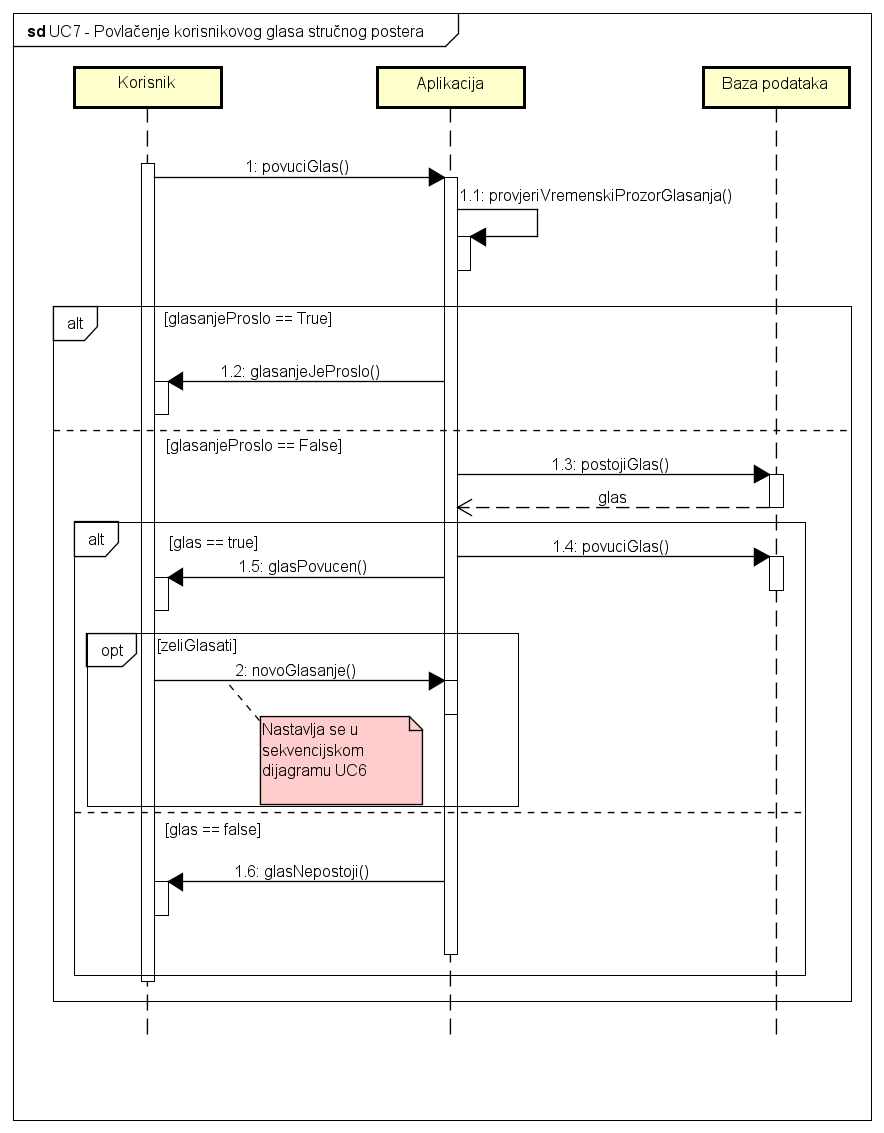
\includegraphics[width=\textwidth]{slike/uc7Sekvencijski.PNG} %veličina u odnosu na širinu linije
					\caption{Sekvencijski dijagram obrasca UC7: Povlačenje korisnikovog glasa stručnog postera}
					\label{fig:uc7-sekvencijski} %label mora biti drugaciji za svaku sliku
				\end{figure}
				
		\section{Ostali zahtjevi}
		 
			  \begin{packed_item}
			 	\item Unutar sustava mora biti omogućen istovremeni rad svih korisnika samog sustava
			 	\item Aplikacija se mora moći koristiti unutar bilo kojeg web-preglednika 
			 	\item Aplikacija se mora ostvariti objektno orijentiranim pristupom programiranja
			 	\item Aplikacija mora biti jednostavna i intuitivna za korištenje svim korisnicima svih uzrasta i predznanja
			 	\item Aplikacija mora biti javno dostupna
			 	\item Unutar aplikacije mora se provoditi autentifikacija te prikazani sadržaj mora odgovarati dozvoljenom sadržaju za trenutnog korisnika
			 	\item Nadogradnjom postojeće aplikacije ne smije doći do urušavanja funkcionalnosti i kvalitete već postojeće aplikacije
			 	\item Unutar sustava mora biti omogućen unos svih posebnih slova referentnih za odabrani jezik aplikacija (za slučaj hrvatskog jezika, mora biti moguć unos dijakritičkih znakova)
			 \end{packed_item}
			 
			 
			 
	
	\chapter{Arhitektura i dizajn sustava}

		{ Arhitektura sustava je hijerarhijska, dakle svaki pojedini sloj
			komunicira isključivo sa slojevima koji su neposredno ispred i iza njega. Slojevi sustava koji mi implementiramo jesu:}
	\begin{itemize}
		\item 	\textit{Korisničko sučelje}
		\item 	\textit{Kontroler}
		\item 	\textit{Servis}
		\item 	\textit{Repozitorij}
		\item 	\textit{Baza podataka}		
	\end{itemize}
	
		{Korisničko sučelje (eng. User interface, UI) predstavlja interaktivno područje između korisnika i računala. Njegov glavni cilj je omogućiti korisnicima učinkovito korištenje i upravljanje računalom te osigurati da računalo pruži korisniku potrebne informacije.\\
			
			Za izradu korisničkog sučelja u ovom slučaju korišten je React, JavaScript biblioteka koja omogućava brzo i jednostavno stvaranje interaktivnih korisničkih sučelja. Kroz korisničko sučelje, korisnik šalje zahtjeve kontroleru, a kontroler potrebne podatke prosljeđuje pomoću JSON (JavaScript Object Notation) datoteka.\\
			
			JSON datoteke služe za pohranu i prijenos podataka u obliku ključ-vrijednost. Nakon što korisničko sučelje preda JSON datoteku, ono očekuje odgovor od kontrolera koji će također biti u JSON formatu. Kontroler u ovom slučaju predstavlja REST API (representational state transfer) te obrađuje zahtjeve vanjskih potrošača.\\
			
			Servis je odgovoran za obradu podataka koje prima od korisničkog sučelja putem kontrolera i baze podataka putem repozitorija. Osim toga, servis obuhvaća poslovne odluke, autorizaciju te provjeru valjanosti identiteta korisnika.\\
			
			Repozitorij ima ulogu komunikacije s bazom podataka te uključuje funkcije za pronalaženje određenih objekata ili skupina objekata iz baze podataka. Ove funkcije obično vraćaju popis objekata koji zadovoljavaju određeni uvjet.\\
			
			Baza podataka koristi se za pohranu i upravljanje podacima te predstavlja ključni dio sustava koji omogućuje trajno čuvanje informacija.\\
			
			Kontroler, servis i repozitorij implementirani su pomoću Java Spring Boota, te su pisani u jeziku JavaScript.}

				
		\section{Baza podataka}
			
		Za potrebe sustava koji implementiramo koristit ćemo se relacijskom bazom podataka koja kao svoju glavnu namjenu ima olakšano modeliranje stvarnog svijeta oko nas. Gradivna jedinica baze jest relacija (tablica) koja je definirana svojim imenom te skupom atributa. Baza podataka ove aplikacije sastoji se od sljedećih entiteta:
		\begin{itemize}
		\item 	\textit{Konferencija}
		\item 	\textit{Korisnik}
		\item 	\textit{Poster}
		\item 	\textit{FotoMaterijal}
		\item 	\textit{PromoMaterijal}		
	\end{itemize}
		
			\subsection{Opis tablica}
			

				{Konferencija - centralni entitet koji definira događaj kojemu pristupaju sudionici, bilo autori ili ne. Atributi koje posjeduje su konfID, kod (za pristup posterima koji su u natjecanju), datPocetak, datKraj, nazivKonf, mjestoKonf, opisKonf}
				
				
				\begin{longtblr}[
					label=none,
					entry=none
					]{
						width = \textwidth,
						colspec={|X[6,l]|X[10, l]|X[20, l]|}, 
						rowhead = 1,
					} %definicija širine tablice, širine stupaca, poravnanje i broja redaka naslova tablice
					\hline \SetCell[c=3]{c}{\textbf{Konferencija}}	 \\ \hline[3pt]
					\SetCell{LightGreen}konfID & INT	&  	Jedinstveni identifikator konferencije  	\\ \hline
					kod	& INT & Pristupna lozinka za posjetitelje  	\\ \hline 
					vrijemePoc & LOCALDATETIME & Vrijeme početka konferencije \\ \hline 
					vrijemeKraj & LOCALDATETIME	& Vrijeme kraja konferencije 		\\ \hline 
					nazivKonf & VARCHAR	& Naziv konferencije 		\\ \hline
					opisKonf & VARCHAR	& Opis konferencije 		\\ \hline
					\SetCell{LightBlue} pbr	& INT &   	Poštanski broj mjesta održavanja konferencije\\ \hline 
				\end{longtblr}
				
				{Mjesto - entitet koji definira mjesto u kojemu se održava konferencija. Atributi koje posjeduje su pbr kao glavni ključ, nazivMjesta, ulica, kućBroj}
				
				
				\begin{longtblr}[
					label=none,
					entry=none
					]{
						width = \textwidth,
						colspec={|X[6,l]|X[6, l]|X[20, l]|}, 
						rowhead = 1,
					} %definicija širine tablice, širine stupaca, poravnanje i broja redaka naslova tablice
					\hline \SetCell[c=3]{c}{\textbf{Mjesto}}	 \\ \hline[3pt]
					\SetCell{LightGreen}pbr & INT	&  	Poštanski broj mjesta održavanja konferencije  	\\ \hline
					nazivMjesta	& VARCHAR & Naziv mjesta gdje se održava konferencija  	\\ \hline 
					ulica & VARCHAR & Ulica u kojoj će se održavati konferencija \\ \hline 
					kućBroj & INT	& Kućanski broj ulice u kojoj će se održavati konferencija  		\\ \hline 
				\end{longtblr}
				
				
				
				
				{FotoMaterijal - entitet FotoMaterijal koristi nam kako bismo mogli pohraniti fotografije nastale tijekom konferencije te ih kasnije prikazati korisnicima. Sadrži entitete: fotoID, nazivFoto, fotoPath te strani ključ konfID pomoću kojega možemo upariti kojoj konferenciji pripada koja fotografija.}
				
	
				\begin{longtblr}[
					label=none,
					entry=none
					]{
						width = \textwidth,
						colspec={|X[6,l]|X[6, l]|X[20, l]|}, 
						rowhead = 1,
					}
					\hline \SetCell[c=3]{c}{\textbf{FotoMaterijal}}	 \\ \hline[3pt]
					\SetCell{LightGreen}fotoID & INT	&  Jedinstveni identifikator fotografije	\\ \hline
					nazivFoto	& VARCHAR &   Naziv fotografije\\ \hline 
					fotoPath & VARCHAR &   Putanja do izvora fotografije\\ \hline 
					\SetCell{LightBlue} konfID	& INT &   	Jedinstveni identifikator konferencije\\ \hline 
				\end{longtblr}
				
				
				{Korisnik - entitet kojim se pokriva registrirani korisnik, neregistrirani korisnik te autor. Sadrži atribute email te lozinka kojima se kasnije može pristupiti posebnom sadržaju specifičnom za registrirane korisnike. Također sadrži ime i prezime i ulogaID koji je strani ključ preko kojeg znamo koju ulogu ima korisnik}
				
				
				\begin{longtblr}[
					label=none,
					entry=none
					]{
						width = \textwidth,
						colspec={|X[6,l]|X[6, l]|X[20, l]|}, 
						rowhead = 1,
					} %definicija širine tablice, širine stupaca, poravnanje i broja redaka naslova tablice
					\hline \SetCell[c=3]{c}{\textbf{Korisnik}}	 \\ \hline[3pt]
					\SetCell{LightGreen}email & VARCHAR	&  Elektronička pošta korisnika	\\ \hline
					lozinka	& VARCHAR &  Lozinka za prijavu korisnika	\\ \hline 
					ime	& VARCHAR &  Ime korisnika	\\ \hline 
					prezime	& VARCHAR &  Prezime korisnika	\\ \hline 
					\SetCell{LightBlue} ulogaID	& INT &   	Jedinstveni identifikator uloge\\ \hline
				\end{longtblr}
				
				{Uloge - entitet kojim se pokrivaju koje uloge sve postoje kao i koje uloge imaju korisnici. Atributi koje sadrži entitet Uloge su: ulogaID koji je glavni ključ i uloga koji opisuje o kojoj je ulozi riječ}
				
				
				\begin{longtblr}[
					label=none,
					entry=none
					]{
						width = \textwidth,
						colspec={|X[6,l]|X[6, l]|X[20, l]|}, 
						rowhead = 1,
					} %definicija širine tablice, širine stupaca, poravnanje i broja redaka naslova tablice
					\hline \SetCell[c=3]{c}{\textbf{Uloge}}	 \\ \hline[3pt]
					\SetCell{LightGreen}ulogaID & ID	&  Jedinstveni identifikator uloge	\\ \hline
					uloga	& VARCHAR &  Uloga korisnika	\\ \hline 
				\end{longtblr}
				
				{Poster - ovim entitetom kontrolirat će se radovi koje na konferenciju dostavljaju autori te se na njoj izlažu i za njih se može glasati. Njegovi atributi su: posterID, nazivPoster, posterPath, email, imeAutor, prezimeAutor, brojGlasova i konfID koji je ujedno i strani ključ pomoću kojega možemo upariti kojoj konferenciji pripada koji poster.}
				
				
				\begin{longtblr}[
					label=none,
					entry=none
					]{
						width = \textwidth,
						colspec={|X[6,l]|X[6, l]|X[20, l]|}, 
						rowhead = 1,
					} %definicija širine tablice, širine stupaca, poravnanje i broja redaka naslova tablice
					\hline \SetCell[c=3]{c}{\textbf{Poster}}	 \\ \hline[3pt]
					\SetCell{LightGreen}posterID & INT	&  	Jedinstveni identifikator postera\\ \hline
					nazivPoster	& VARCHAR &   Naziv postera	\\ \hline 
					posterPath & VARCHAR &   Putanja do izvora postera\\ \hline 
					email	& VARCHAR &   Elektronička pošta korisnika\\ \hline
					imeAutor & VARCHAR &   Ime autora postera\\ \hline 
					prezimeAutor & VARCHAR &   Prezime autora postera\\ \hline 
					brojGlasova & INT &   Ostvareni broj glasova postera\\ \hline 
					\SetCell{LightBlue} konfID	& INT &  Jedinstveni identifikator konferencije	\\ \hline 
				\end{longtblr}
				
				{PromoMaterijal - entitet PromoMaterijal pokriva konkretan ponuđeni materijal kojemu registrirani korisnik može pristupiti. Atributi koje ima su promoID, nazivPromo, url, promoPath i konfID koji je ujedno i strani ključ pomoću kojega možemo upariti kojoj konferenciji pripada koji promotivni materijal.}
				 
				
				\begin{longtblr}[
					label=none,
					entry=none
					]{
						width = \textwidth,
						colspec={|X[6,l]|X[6, l]|X[20, l]|}, 
						rowhead = 1,
					} %definicija širine tablice, širine stupaca, poravnanje i broja redaka naslova tablice
					\hline \SetCell[c=3]{c}{\textbf{PromoMaterijal}}	 \\ \hline[3pt]
					\SetCell{LightGreen}posterID & INT	&  Jedinstveni identifikator postera\\ \hline
					nazivPromo	& VARCHAR &   Naziv promotivnog materijala	\\ \hline 
					promoPath & VARCHAR &  Putanja do izvora sadržaja promotivnog materijala \\ \hline
					url & VARCHAR &  WEB stranica pokrovitelja \\ \hline
					\SetCell{LightBlue} konfID	& INT &   Jedinstveni identifikator konferencije	\\ \hline   
				\end{longtblr}
				
				{Glasanje - entitet Glasanje služi za prebrojavanje broja glasova postera te također služi za prevenciju glasovanja jednog registriranog korisnika za više postera. Atributi koji sadrži entitet Glasanje su: posterID koji je jedinstveni identifikator postera te je također i primarni ključ, konfID koji je jedinstveni identifikator konferencije te je također i strani ključ email koji je elektronička pošta korisnika ali je isto tako i strani ključ}
				
				
				\begin{longtblr}[
					label=none,
					entry=none
					]{
						width = \textwidth,
						colspec={|X[6,l]|X[6, l]|X[20, l]|}, 
						rowhead = 1,
					} %definicija širine tablice, širine stupaca, poravnanje i broja redaka naslova tablice
					\hline \SetCell[c=3]{c}{\textbf{Glasanje}}	 \\ \hline[3pt]
					\SetCell{LightGreen}posterID & INT	&  Jedinstveni identifikator postera\\ \hline
					\SetCell{LightBlue} konfID	& INT &   Jedinstveni identifikator konferencije	\\ \hline 
					\SetCell{LightBlue} email	& VARCHAR &   Elektronička pošta korisnika	\\ \hline   
				\end{longtblr}
				
				
			
			\subsection{Dijagram baze podataka}
					\begin{figure}[H]
					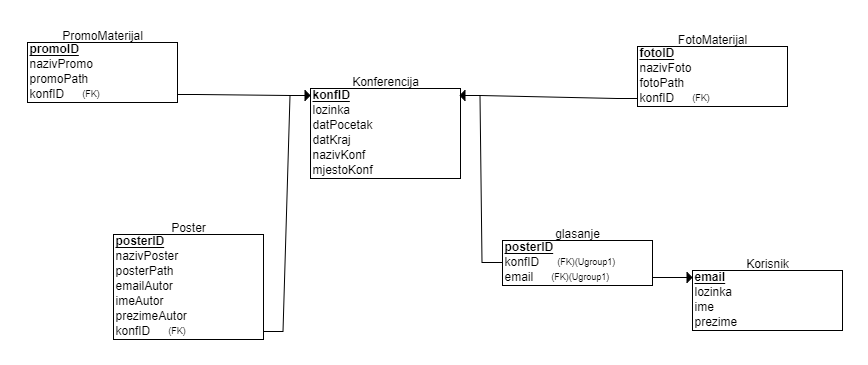
\includegraphics[width=\textwidth]{slike/bazaPodataka.PNG} %veličina u odnosu na širinu linije
					\caption{Dijagram baze podataka}
					\label{fig:promjene4} %label mora biti drugaciji za svaku sliku
				\end{figure}
			
			\eject
			
			
		\section{Dijagram razreda}
		

			
			
			
			\eject
		
		\section{Dijagram stanja}
			
			
			\textbf{\textit{dio 2. revizije}}\\
			
			\textit{Potrebno je priložiti dijagram stanja i opisati ga. Dovoljan je jedan dijagram stanja koji prikazuje \textbf{značajan dio funkcionalnosti} sustava. Na primjer, stanja korisničkog sučelja i tijek korištenja neke ključne funkcionalnosti jesu značajan dio sustava, a registracija i prijava nisu. }
			
			
			\eject 
		
		\section{Dijagram aktivnosti}
			
			\textbf{\textit{dio 2. revizije}}\\
			
			 \textit{Potrebno je priložiti dijagram aktivnosti s pripadajućim opisom. Dijagram aktivnosti treba prikazivati značajan dio sustava.}
			
			\eject
		\section{Dijagram komponenti}
		
			\textbf{\textit{dio 2. revizije}}\\
		
			 \textit{Potrebno je priložiti dijagram komponenti s pripadajućim opisom. Dijagram komponenti treba prikazivati strukturu cijele aplikacije.}
	\chapter{Implementacija i korisničko sučelje}
		
		\section{Korištene tehnologije i alati}
		
			 
			 Za izradu projekta koristili smo različite tehnologije, alate i platforme kako bismo učinkovito surađivali i razvili visokokvalitetnu aplikaciju. Za međusobnu komunikaciju unutar tima koristili smo aplikacije WhatsApp\footnote{\url{https://www.whatsapp.com/}} i Discord\footnote{\url{https://discord.com/}} što nam je omogućilo brz i jednostavan način dijeljenja informacija i dogovaranja.
			 
			 Sustav za upravljanje izvornim kodom bio je Git\footnote{\url{https://git-scm.com/}}, a repozitorij projekta smješten je na web platformi GitHub\footnote{\url{https://github.com/}}. Ovo nam je omogućilo sinkronizaciju rada, praćenje promjena i suradnju na kodu na učinkovit način. Za izradu UML dijagrama korišten je alat Astah UML\footnote{\url{https://astah.net/products/astah-uml/}}, pružajući jasnu vizualizaciju strukture i odnosa unutar projekta.
			 
			 Integrirano razvojno okruženje (IDE) koje smo koristili bilo je IntelliJ\footnote{\url{https://www.jetbrains.com/idea/}}, razvijeno u tvrtki JetBrains. IntelliJ je posebno prilagođen za rad s računalnim softverom napisanim u Javi, Kotlinu i Groovyju te pruža potporu za druge popularne jezike kao što su Python, JavaScript i TypeScript. To osigurava dosljedno iskustvo rada na različitim operativnim sustavima - Windows, macOS i Linux.
			 
			 Za backend aplikacije koristili smo Spring Boot\footnote{\url{https://spring.io/projects/spring-boot/}}, radni okvir baziran na Javi koji nudi autokonfiguraciju za olakšavanje početka razvoja, ali istovremeno omogućuje programerima da prilagode konfiguraciju prema potrebama.
			 
			 Frontend je implementiran pomoću Reacta\footnote{\url{https://react.dev/}}, biblioteke u JavaScriptu\footnote{\url{https://www.javascript.com/}} za izgradnju korisničkih sučelja. React se temelji na komponentama što je omogućilo razvoj složenih aplikacija s jasnom strukturom.\\
			 
			 Baza podataka projekta bila je PostgreSQL\footnote{\url{https://www.postgresql.org/}}, otvoreni sustav za upravljanje relacijskom bazom podataka. Konačno, aplikacija se nalazi na Renderu\footnote{\url{https://render.com/}}, oblak platformi kao usluzi, koja podržava različite programske jezike i omogućuje laku implementaciju i upravljanje modernim aplikacijama.
			 
			 Za ispitivanje sustava korišten je radni okvir Selenium\footnote{\url{https://www.seleniumhq.org/}} koji pruža automatsko testiranje kako bi se osigurala funkcionalnost i stabilnost sustava.
			 
			 Kombinacija ovih tehnologija i alata omogućila je timu učinkovit rad i uspješan razvoj aplikacije.
			
			
			\eject 
		
	
		\section{Ispitivanje programskog rješenja}
		
			 
			 Ispitivanje programskog riješena proveli smo na dva načina:
			 \begin{itemize}
			 	\item \textit{Ispitivanje komponenti - ostvareno pomoću JUnit testova u programskom jeziku Java}
			 	\item \textit{Ispitivanje sustava - ostvareno pomoću Selenium alata za automatizirano testiranje web aplikacija}
			 \end{itemize}
			 	
			 
			 
	
			
			\subsection{Ispitivanje komponenti}
			Ispitivanje komponenti bazira se na ispitivanjima funkcija programa kao što su broj poziva određene funkcije, šta točno vraćaju funkcije nakon što se izvedu, izaziva li se neka iznimka...
			
			\begin{packed_enum}
				\item Prvo testiranje testira kreiranje korisnika
				
				\begin{quote}
						Provjeravamo funkcionalnost funkcija za kreiranje korisnika te koliko puta se koja funkcija pozvala.
						\begin{figure}[H]
							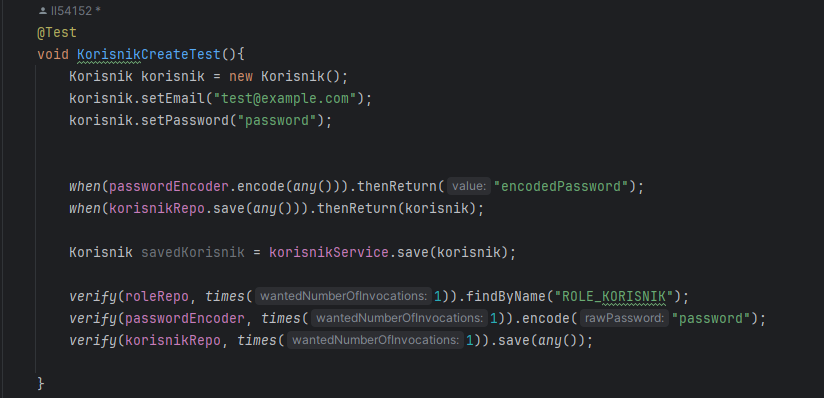
\includegraphics[width=\textwidth]{slike/JUnit1.png} %veličina u odnosu na širinu linije
							\caption{Prvo testiranje}
							\label{fig:JUnit1} %label mora biti drugaciji za svaku sliku
						\end{figure}
				\end{quote}
				
				
				\item Drugo testiranje testira ulazak u konferenciju
				
				\begin{quote}
					U drugom testiranju provjeravamo ulazak u konferenciju kao i sve funkcionalnosti vezanu uz nju.
					\begin{figure}[H]
						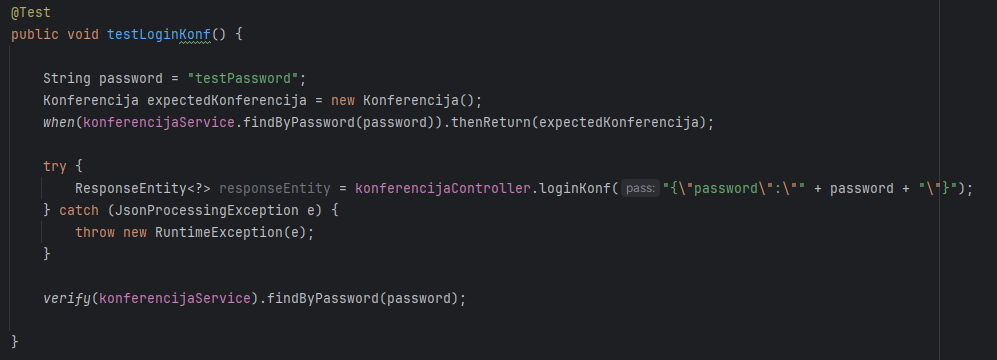
\includegraphics[width=\textwidth]{slike/JUnit2.png} %veličina u odnosu na širinu linije
						\caption{Drugo testiranje}
						\label{fig:JUnit2} %label mora biti drugaciji za svaku sliku
					\end{figure}
				\end{quote}
				
				\item Treće testiranje testira neuspješan ulazak u konferenciju
				\begin{quote}
					U trećem testiranju provjeravamo ponašanje naše aplikacije u slučaju neuspjelog ulaska u konferenciju kao i sve funkcionalnosti vezanu uz nju.
					\begin{figure}[H]
						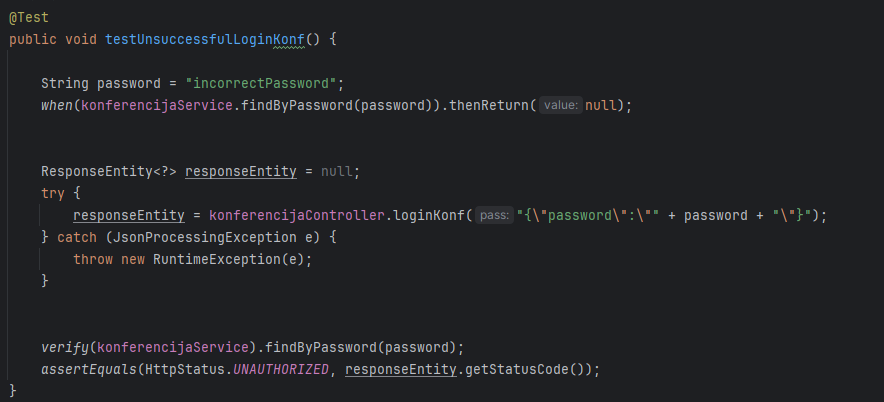
\includegraphics[width=\textwidth]{slike/JUnit3.png} %veličina u odnosu na širinu linije
						\caption{Treće testiranje}
						\label{fig:JUnit3} %label mora biti drugaciji za svaku sliku
					\end{figure}
				\end{quote}
				
				\item Četvrto testiranje testira dohvat svih konferencija 
				\begin{quote}
					U četvrtom testiranju testiramo funkcionalnost dohvaćanja svih konferencija budući da je to jedna od ključnih funkcija prilikom kreiranja konferencije.
					\begin{figure}[H]
						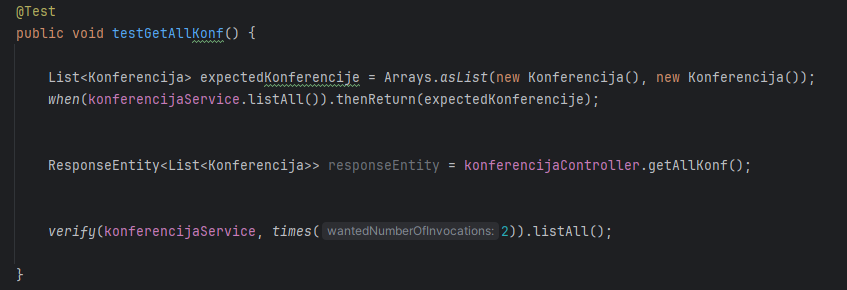
\includegraphics[width=\textwidth]{slike/JUnit4.png} %veličina u odnosu na širinu linije
						\caption{Četvrto testiranje}
						\label{fig:JUnit4} %label mora biti drugaciji za svaku sliku
					\end{figure}
				\end{quote}
				
				\item Peto testiranje testira dohvat svih lokacije
				\begin{quote}
					U petom testiranju testiramo funkcionalnost dohvaćanja lokacije koja je ključna za prikaz karte i vremenske prognoze.
					\begin{figure}[H]
						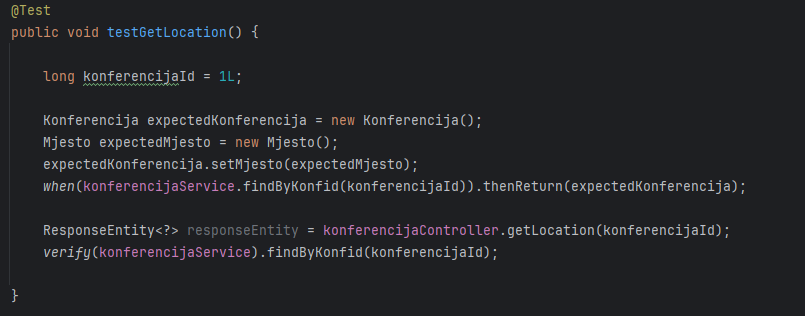
\includegraphics[width=\textwidth]{slike/JUnit5.png} %veličina u odnosu na širinu linije
						\caption{Peto testiranje}
						\label{fig:JUnit5} %label mora biti drugaciji za svaku sliku
					\end{figure}
				\end{quote}
				
				\item Šesto testiranje testira kreiranje mjesta uz konferenciju
				\begin{quote}
					U šestom testiranju testiramo funkcionalnost kreiranja i dodavanja mjesta nekoj konferenciji.
					\begin{figure}[H]
						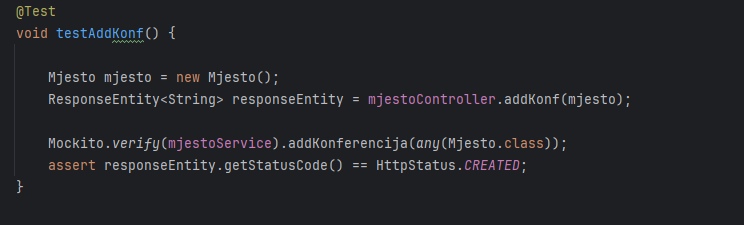
\includegraphics[width=\textwidth]{slike/JUnit6.png} %veličina u odnosu na širinu linije
						\caption{Šesto testiranje}
						\label{fig:JUnit6} %label mora biti drugaciji za svaku sliku
					\end{figure}
				\end{quote}
				
			\begin{figure}[H]
				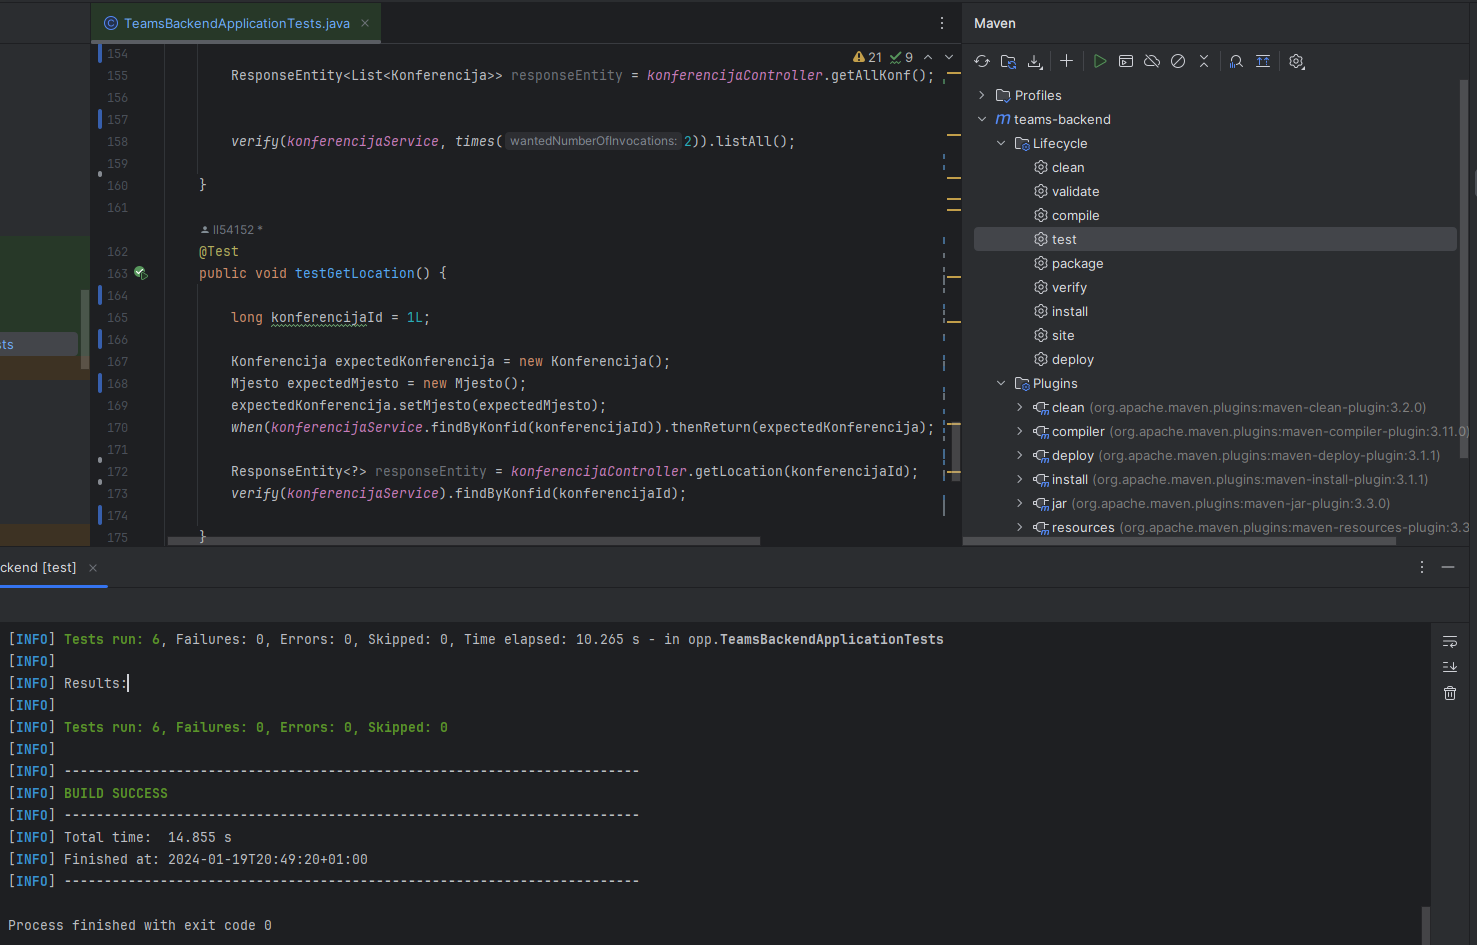
\includegraphics[width=\textwidth]{slike/JUnitAll.png} %veličina u odnosu na širinu linije
				\caption{Rezultati testova}
				\label{fig:JUnitAll} %label mora biti drugaciji za svaku sliku
			\end{figure}
			
				
			\end{packed_enum}
			
			
			
			\subsection{Ispitivanje sustava}
			Ispitivanje sustava smo proveli koristeći Selenium WebDriver i zadnju verziju FireFox web preglednika. Selenium smo konfigurirali pomoću programskog jezika Java te je onda Selenium automatizirano testirao našu aplikaciju bazirajući se na naše testove. Za Selenium testiranje smo bili isključili reCAPTCHA.
	
			
			\begin{packed_enum}
				\item Prvo testiranje testira registraciju korisnika
				
				\begin{quote}
					Provjeravamo funkcionalnost registracije korisnika. U polja upisujemo podatke te se pritišće gumb nakon upisa. Ukoliko je test prošao, korisnik je uspješno stvoren i prijavljen u aplikaciju.
					\begin{figure}[H]
						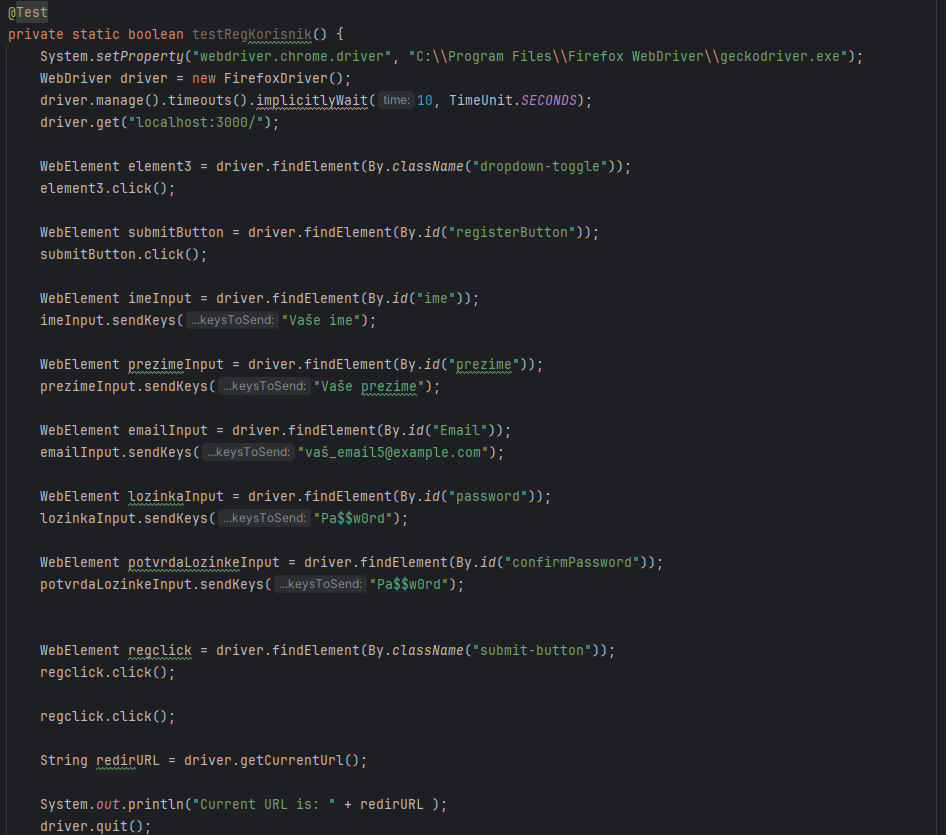
\includegraphics[width=\textwidth]{slike/Selenium1.png} %veličina u odnosu na širinu linije
						\caption{Prvo testiranje}
						\label{fig:Selenium1} %label mora biti drugaciji za svaku sliku
					\end{figure}
				\end{quote}
				
				
				\item Drugo testiranje testira dodavanje konferencije
				
				\begin{quote}
					U drugom testiranju provjeravamo dodavanje konferencije. Prije samog dodavanja konferencije, administrator se mora prijaviti u sustav te nakon prijave, administrator upisuje podatke za konferenciju te pritišće gumb za dodaju. Ukoliko je test prošao, konferencija će biti dodana te će se prikazati poruka o uspješnosti našeg dodavanja.
					\begin{figure}[H]
						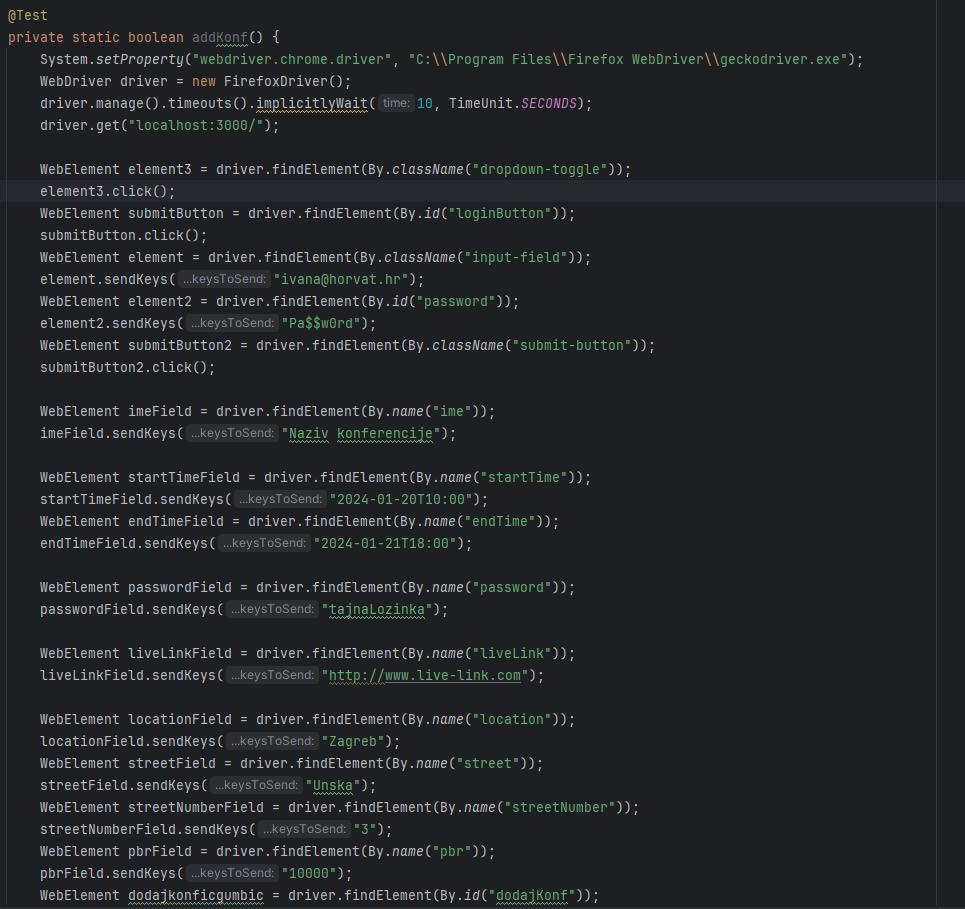
\includegraphics[width=\textwidth]{slike/Selenium2.png} %veličina u odnosu na širinu linije
						\caption{Drugo testiranje}
						\label{fig:Selenium2} %label mora biti drugaciji za svaku sliku
					\end{figure}
				\end{quote}
				
				\item Treće testiranje testira prijavu korisnika
				\begin{quote}
					U trećem testiranju provjeravamo prijavu korisnika. U prazna polja upisujemo potrebne podatke te na kraju pritišćemo gumb za prijavu. Ukoliko je test uspješan, vratit će nas na početnu stranicu.
					\begin{figure}[H]
						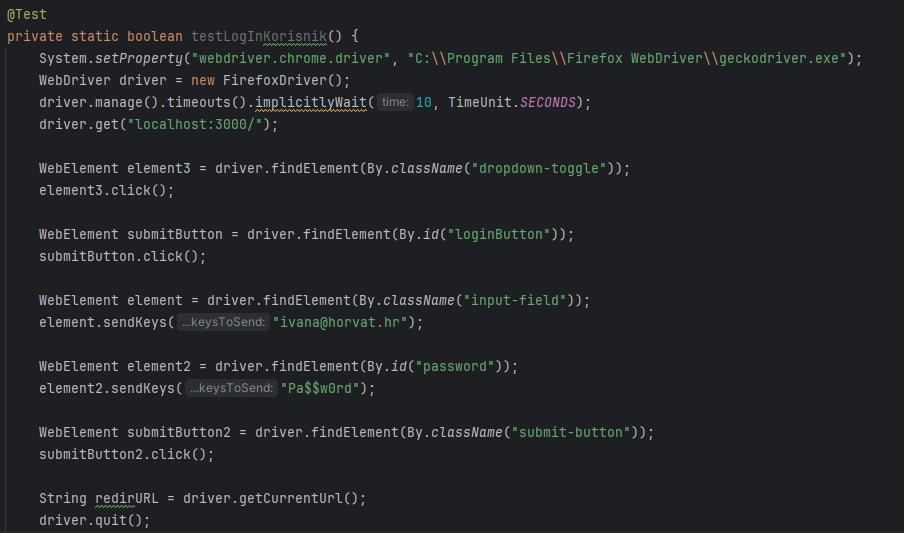
\includegraphics[width=\textwidth]{slike/Selenium3.png} %veličina u odnosu na širinu linije
						\caption{Treće testiranje}
						\label{fig:Selenium3} %label mora biti drugaciji za svaku sliku
					\end{figure}
				\end{quote}
				
				\item Četvrto testiranje testira prijavu u konferenciju 
				\begin{quote}
					U četvrtom testiranju testiramo prijavu u konferenciju. Unutar polja za unos lozinke, upisujemo lozinku i pritišćemo gumb za prijavu. Ukoliko je test uspješan, aplikacija će nas vratiti na početnu stranicu konferencije.
					\begin{figure}[H]
						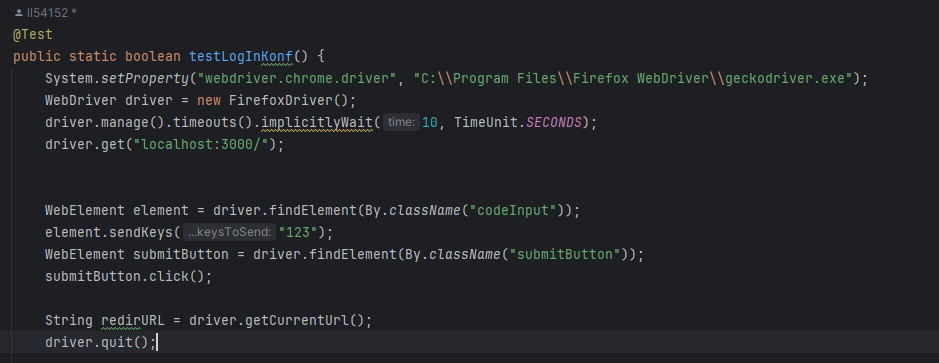
\includegraphics[width=\textwidth]{slike/Selenium4.png} %veličina u odnosu na širinu linije
						\caption{Četvrto testiranje}
						\label{fig:Selenium4} %label mora biti drugaciji za svaku sliku
					\end{figure}
				\end{quote}
				
			\end{packed_enum}
			
			\begin{figure}[H]
				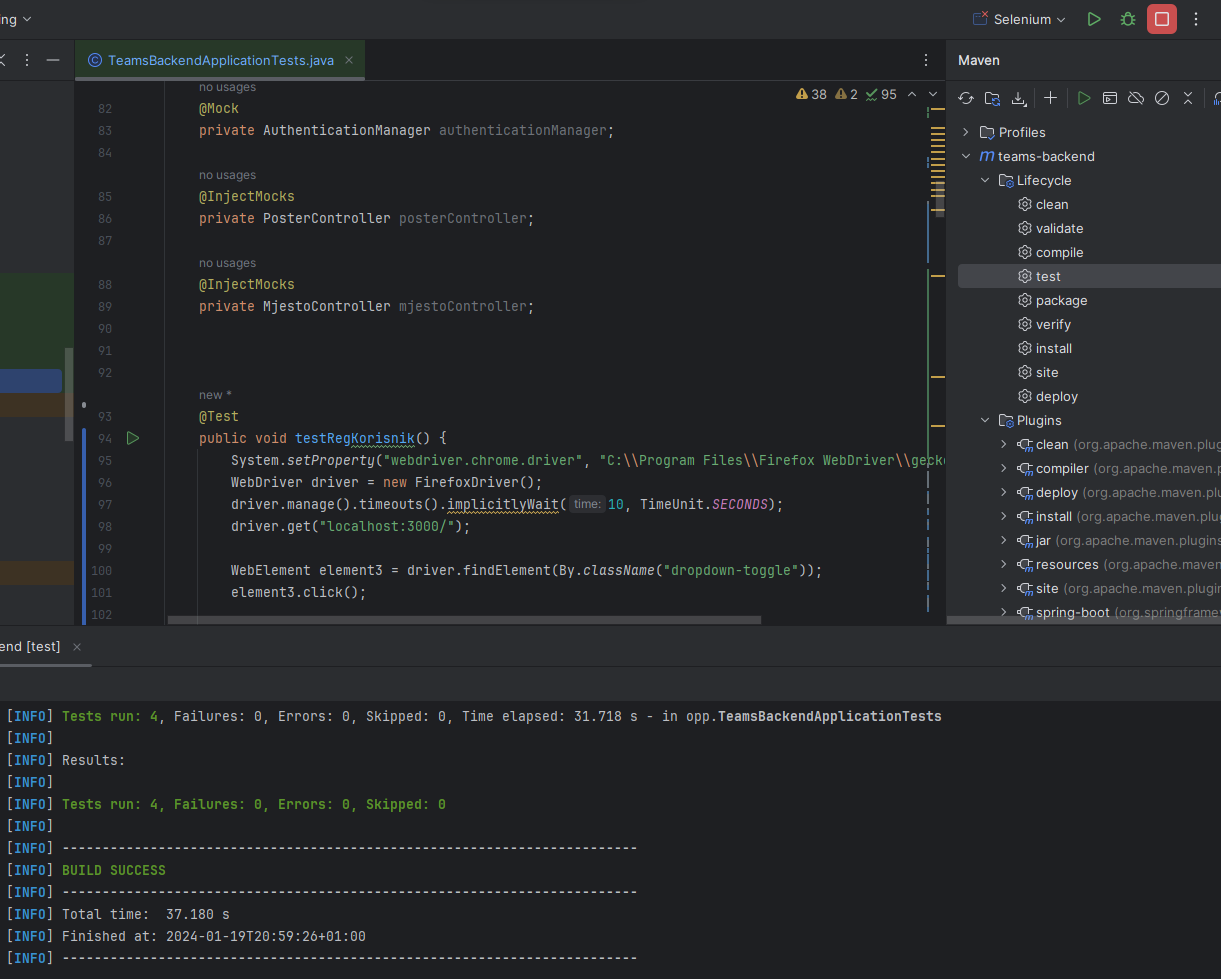
\includegraphics[width=\textwidth]{slike/SeleniumAll.png} %veličina u odnosu na širinu linije
				\caption{Rezultati testova}
				\label{fig:SeleniumAll} %label mora biti drugaciji za svaku sliku
			\end{figure}
			
			\eject 
		
		
		\section{Dijagram razmještaja}
			
			Dijagram razmještaja~\ref{fig:dijagramRazmjestaja} opisuje topologiju sklopovlja i programsku potporu koja se koristi u implementaciji sustava u njegovom radnom okruženju. Sustav je baziran na arhitekturi "klijent-poslužitelj". Poslužiteljsko računalo (Render) sadrži web poslužitelj na kojem se nalazi naša web aplikacija te sadrži poslužitelj baze podataka na kojemu je naša Postgres baza podataka. Komunikacija između klijenta i poslužitelja obavlja se preko sigurnog kanala ostvarenog protokolom HTTPS.
			
			
			 \begin{figure}[H]
				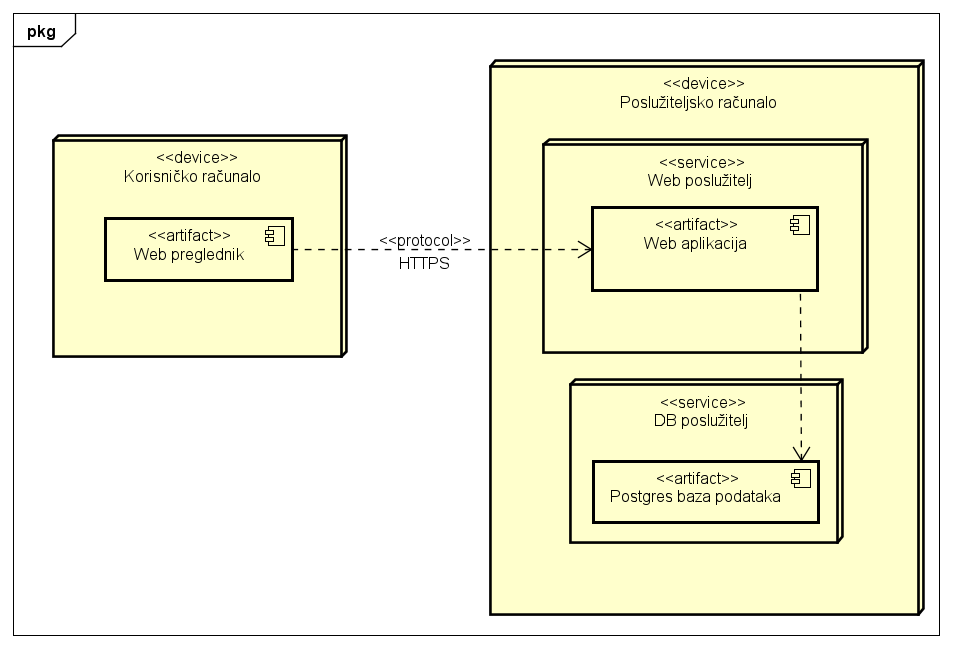
\includegraphics[width=\textwidth]{slike/dijagramRazmjestaja.PNG} %veličina u odnosu na širinu linije
				\caption{Dijagram razmještaja}
				\label{fig:dijagramRazmjestaja} %label mora biti drugaciji za svaku sliku
			\end{figure}
			
			
			\eject 
		
		\section{Upute za puštanje u pogon}
		
			Za puštanje aplikacije u pogon (eng. deployment) koristili smo web stranicu Render.
			Prema uputama danim na GitHub repozitoriju tvrtke CROZ (https://github.com/progi-devops/) pripremili smo naš sustav za puštanje u pogon.
			Kako bismo mogli koristiti usluge servisa Render, prvotno smo se morali prijaviti u sustav, a to smo učinili s pomoću istih podataka s kojima smo stvorili GitHub repozitoriji na kojemu držimo i održavamo naš projekt te njegov kod. Prvotno se podiže virtualna baza, a nakon nje potrebno je namjestiti skripte koje se izvode (navedene u package.json dokumentu i Dockerfile dokumentu) prilikom izgradnje rješenja projekta te prilikom samog pokretanja tog izgrađenog rješenja. To vrijedi i za pripremu "backend" i "frontend" dijela. Također, za "frontend" dio, u uputama se mogu pronaći koraci kako osigurati neometano lokalno pokretanje aplikacije bez obzira na novo-dodane datoteke. Pri podizanju baze nije potrebno unositi gotovo nikakve podatke, već samo vrstu bazu kojom se koristimo (u našem slučaju PostgreSQL) te vremensku zonu kojoj pripadamo. Nakon toga Render nam povratno pruža sve potrebne informacije koje nam trebaju za lokalno spajanje na virtualnu bazu te povezivanje "backend"-a na nju. Nakon toga moramo pustiti u pogon "backend" dio aplikacije kako bismo dobili URL na koji će naš "frontend", pušten u pogon, slati zahtjeve i s kojega će primati odgovore. Dockerfile koji nam je potreban za puštanje u pogon kreirali smo po uzoru na dani Dockerfile sa već spomenutog GitHub repozitorija, uz manje preinake kod podataka vezanih za povezivanje na bazu. Isto vrijedi za package.json dokument te app.js. Također, bitno je istaknuti da Render prilikom puštanja u pogon koristi prethodno zadanu granu s odabranog repozitorija s koje potom uzima kod koji konkretno pušta u pogon. Tako prilikom svakog novog postavljanja promjena (eng. commit and push) na odabranu granu, na Render servisu automatski se ponovno pušta u pogon kompletna aplikacija (osim baze podataka) s novim promjenama.
			
			\begin{figure}[H]
				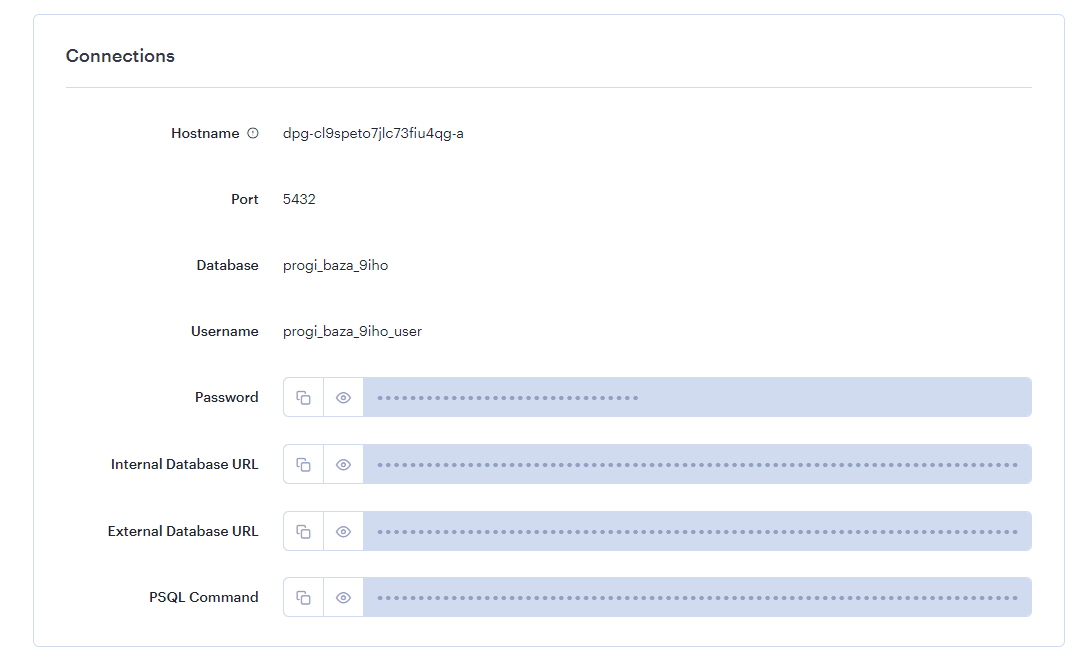
\includegraphics[width=\textwidth]{slike/DB_podatci.png} %veličina u odnosu na širinu linije
				\caption{Generirani podatci za povezivanje na bazu}
				\label{fig:DB_podatci} %label mora biti drugaciji za svaku sliku
			\end{figure}
			
			\begin{figure}[H]
				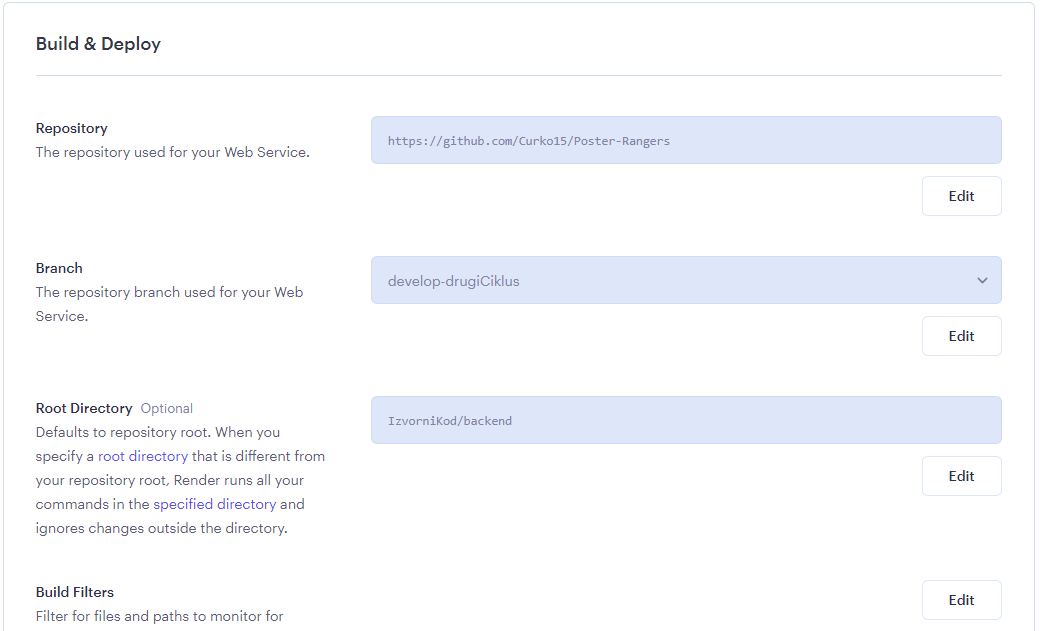
\includegraphics[width=\textwidth]{slike/BE_setup.png} %veličina u odnosu na širinu linije
				\caption{Postavljanje repozitorija, grane te direktorija za "backend"}
				\label{fig:BE_setup} %label mora biti drugaciji za svaku sliku
			\end{figure}
			
			\begin{figure}[H]
				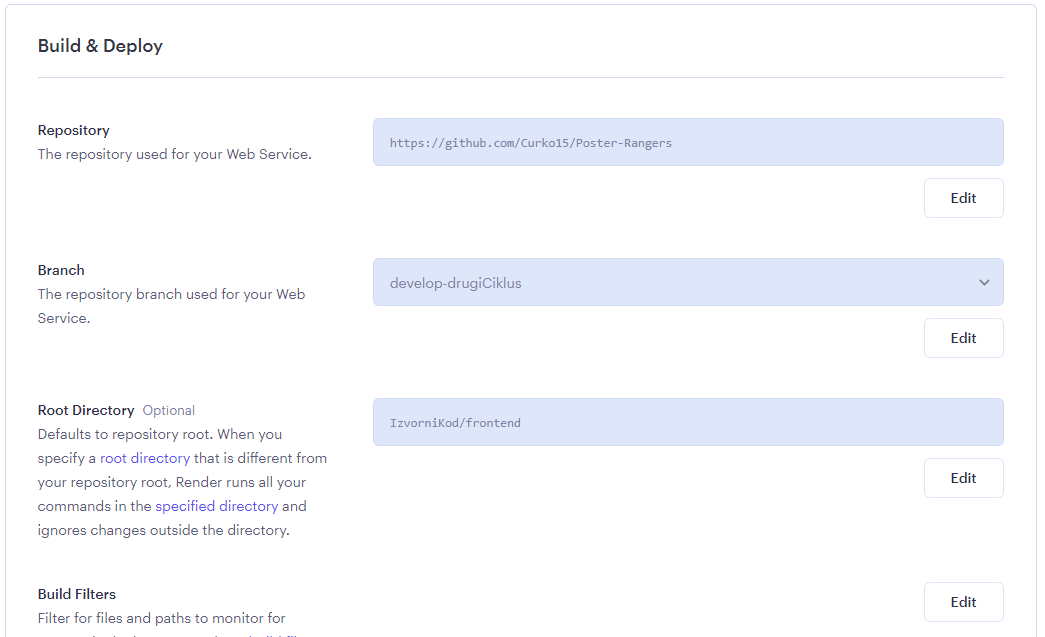
\includegraphics[width=\textwidth]{slike/FE_setup.png} %veličina u odnosu na širinu linije
				\caption{Postavljanje repozitorija, grane te direktorija za "frontend"}
				\label{fig:FE_setup} %label mora biti drugaciji za svaku sliku
			\end{figure}
			
			\begin{figure}[H]
				
\includegraphics[width=\textwidth]{slike/deployed_URL.png} %veličina u odnosu na širinu linije
				\caption{generirani URL za pristup puštenoj aplikaciji}
				\label{fig:deployed_URL} %label mora biti drugaciji za svaku sliku
			\end{figure}
			
			
			\eject 
	\chapter{Zaključak i budući rad}
				
		 
		 Zadatak našeg tima bio je razviti web-aplikaciju za stručne konferencije koja bi organizatorima omogućila veći doseg ljudi budući da bi se na konferenciji moglo sudjelovati i online te bi se u sklopu svake konferencije mogli pregledavati stručni radovi (posteri) drugih ljudi i za te radove glasati. Na projektu smo radili 3 mjeseca i naposljetku ga uspješno završili i ostvarili sve potrebne funkcionalnosti.\\
		 
		 U prvoj fazi projekta, prije samog početka izrade projektnog zadatka, diskutirali smo o njegovoj temi i razmišljali kako najbolje organizirati i razviti aplikaciju. Nakon uspostave plana, izradili smo bazu podataka koja je ključni dio svake aplikacije, krenuli s izradom dokumentacije pa naposljetku i sa samom implementacijom. U ovoj smo fazi implementirali većinu potrebnih funkcionalnost poput prijave, registracije, stvaranja konferencije i admina. Pojedini su članovi imali nešto više programerskog iskustva što je zasigurno pomoglo bržem napretku projekta i drugim članovima tima dalo dovoljno vremena da se uhodaju u svoje zadatke. Prije predaje prve revizije aplikaciju smo postavili na Render što nam je bio jedan od brojnih tehničkih izazova ove faze.

		 U drugoj smo fazi implementirali ostale potrebne funkcionalnosti među kojima su dodavanje i prikaz postera, fotografija i promotivnih materijala. U toj smo se fazi susreli s izazovima oko prikazivanja fotografija, no i taj smo problem riješili i stekli potrebna znanja za ubuduće. Dorađivanjem finesa, testiranjem aplikacije i dovršetkom dokumentacije završili smo sa svojim projektnim zadatkom vrlo zadovoljni učinjenim.
		 
		 Za cijelo vrijeme trajanja izrade projekta, vrlo se bitnom stavkom pokazala međusobna komunikacija i pomoć među članovima tima, redoviti online sastanci i zajedništvo u rješavanju izazova te uključenost našeg voditelja u sve korake procesa.
		 
		 Moguća nadogradnja aplikacije donijela bi korisnicima mogućnost primanja obavijesti o događanjima na konferenciji i davanje feedbacka na cjelokupnu konferenciju, a tijekom vremena zasigurno bi se moglo nadodati još novih funkcionalnosti koje bi korisnicima poboljšale iskustvo prisustvovanja na konferenciji.\\
		 
		 Sudjelovanje u ovom projektu bilo je intenzivno iskustvo koje nam je pružilo dublji uvid u kompleksnosti timskog rada programera. Razvili smo vještine organizacije, suradnje i komunikacije unutar tima. Rad na projektu pružio nam je priliku primijeniti teorijsko znanje u stvarnom okruženju praktičnom primjenom principa programskog inženjerstva. Shvatili smo važnost timskog duha, prilagodbe te jasne komunikacije, a istovremeno smo svjesni prostora za osobni i timski napredak. Za brže i kvalitetnije izvođenje projekata u budućnosti, prepoznajemo potrebu za usavršavanjem u područjima agilnog upravljanja projektima, testiranja softvera te optimizacije koda. Ovo iskustvo postat će temelj našeg profesionalnog razvoja, osiguravajući da budući projekti budu izvedeni s još većim uspjehom.
		 
		 
		 
		 
		 
		 
		
		 
		  
		 
		 
		 
		 
		
		\eject 
	\chapter*{Popis literature}
		\addcontentsline{toc}{chapter}{Popis literature}
	 	
		
		
		\begin{enumerate}
			
			
			\item  Programsko inženjerstvo, FER ZEMRIS, \url{http://www.fer.hr/predmet/proinz}
			
			\item  I. Sommerville, "Software engineering", 8th ed, Addison Wesley, 2007.
			
			\item  T.C.Lethbridge, R.Langaniere, "Object-Oriented Software Engineering", 2nd ed. McGraw-Hill, 2005.
			
			\item  I. Marsic, Software engineering book``, Department of Electrical and Computer Engineering, Rutgers University, \url{http://www.ece.rutgers.edu/~marsic/books/SE}
			
			\item  The Unified Modeling Language, \url{https://www.uml-diagrams.org/}
			
			\item  Astah Community, \url{http://astah.net/editions/uml-new}
		\end{enumerate}
		
		 
	
	
	\begingroup
	\renewcommand*\listfigurename{Indeks slika i dijagrama}
	%\renewcommand*\listtablename{Indeks tablica}
	%\let\clearpage\relax
	\listoffigures
	%\vspace{10mm}
	%\listoftables
	\endgroup
	\addcontentsline{toc}{chapter}{Indeks slika i dijagrama}


	
	\eject 
		
	\chapter*{Dodatak: Prikaz aktivnosti grupe}
		\addcontentsline{toc}{chapter}{Dodatak: Prikaz aktivnosti grupe}
		
		\section*{Dnevnik sastajanja}
		
		\textbf{\textit{Kontinuirano osvježavanje}}\\
		
		 \textit{U ovom dijelu potrebno je redovito osvježavati dnevnik sastajanja prema predlošku.}
		
		\begin{packed_enum}
			\item  sastanak
			
			\item[] \begin{packed_item}
				\item Datum: 18. listopada 2023.
				\item Prisustvovali: D. Bevanda, M.Ćurković, A. Dumančić, K. Jurić, L. Lulić, L. Miličević i F. Talan
				\item Teme sastanka:
				\begin{packed_item}
					\item  rasprava o projektnom zadatku (brainstorming)
					\item  okvirna podjela poslova
				\end{packed_item}
			\end{packed_item}
			
			\item  sastanak
			\item[] \begin{packed_item}
				\item Datum: 20. listopada 2023.
				\item Prisustvovali: D. Bevanda, M. Ćurković, A. Dumančić, K. Jurić, L. Lulić, L. Miličević i F. Talan
				\item Teme sastanka:
				\begin{packed_item}
					\item  detaljno proučavanje zadatka
					\item  okviran dogovor što bi trebalo implementirati
				\end{packed_item}
			\end{packed_item}

            \item  sastanak
			\item[] \begin{packed_item}
				\item Datum: 22. listopada 2023.
				\item Prisustvovali: D. Bevanda, M. Ćurković, L. Lulić i L. Miličević 
				\item Teme sastanka:
				\begin{packed_item}
					\item  dogovor i skica baze podataka
				\end{packed_item}
			\end{packed_item}

            \item  sastanak
			\item[] \begin{packed_item}
				\item Datum: 23. listopada 2023.
				\item Prisustvovali: A. Dumančić, K. Jurić i F. Talan
				\item Teme sastanka:
				\begin{packed_item}
					\item  dogovor oko izgleda korisničkog sučelja i potrebnih funkcionalnosti
				\end{packed_item}
			\end{packed_item}

            \item  sastanak
			\item[] \begin{packed_item}
				\item Datum: 28. listopada 2023.
				\item Prisustvovali: D. Bevanda, M. Ćurković, A. Dumančić, K. Jurić, L. Lulić, L. Miličević i F. Talan
				\item Teme sastanka:
				\begin{packed_item}
					\item  izrada konceptualnog modela baze podataka
				\end{packed_item}
			\end{packed_item}

			\item  sastanak
			\item[] \begin{packed_item}
				\item Datum: 4. studenog 2023.
				\item Prisustvovali: D. Bevanda, M. Ćurković, A. Dumančić, K. Jurić, L. Lulić, L. Miličević i F. Talan
				\item Teme sastanka:
				\begin{packed_item}
					\item  pregled dotad napravljene dokumentacije
                    \item  podjela daljnjih poslova
				\end{packed_item}
			\end{packed_item}
			
			%
			
		\end{packed_enum}
		
		\eject
		\section*{Tablica aktivnosti}
		
			\textbf{\textit{Kontinuirano osvježavanje}}\\
			
			 \textit{Napomena: Doprinose u aktivnostima treba navesti u satima po članovima grupe po aktivnosti.}

			\begin{longtblr}[
					label=none,
				]{
					vlines,hlines,
					width = \textwidth,
					colspec={X[7, l]X[1, c]X[1, c]X[1, c]X[1, c]X[1, c]X[1, c]X[1, c]}, 
					vline{1} = {1}{text=\clap{}},
					hline{1} = {1}{text=\clap{}},
					rowhead = 1,
				} 
			
				\SetCell[c=1]{c}{} & \SetCell[c=1]{c}{\rotatebox{90}{\textbf{Marko Ćurković}}} & \SetCell[c=1]{c}{\rotatebox{90}{\textbf{Daria Bevanda }}} &	\SetCell[c=1]{c}{\rotatebox{90}{\textbf{Andrija Dumančić }}} & \SetCell[c=1]{c}{\rotatebox{90}{\textbf{Korina Jurić }}} &	\SetCell[c=1]{c}{\rotatebox{90}{\textbf{Luka Lulić }}} & \SetCell[c=1]{c}{\rotatebox{90}{\textbf{Luka Miličević }}} &	\SetCell[c=1]{c}{\rotatebox{90}{\textbf{Fran Talan }}} \\  
				Upravljanje projektom 		&  &  &  &  &  &  & \\ 
				Opis projektnog zadatka 	&  &  &  &  &  &  & \\ 
				
				Funkcionalni zahtjevi       &  &  &  &  &  &  &  \\ 
				Opis pojedinih obrazaca 	&  &  &  &  &  &  &  \\ 
				Dijagram obrazaca 			&  &  &  &  &  &  &  \\ 
				Sekvencijski dijagrami 		&  &  &  &  &  &  &  \\ 
				Opis ostalih zahtjeva 		&  &  &  &  &  &  &  \\ 

				Arhitektura i dizajn sustava	 &  &  &  &  &  &  &  \\ 
				Baza podataka				&  &  &  &  &  &  &   \\ 
				Dijagram razreda 			&  &  &  &  &  &  &   \\ 
				Dijagram stanja				&  &  &  &  &  &  &  \\ 
				Dijagram aktivnosti 		&  &  &  &  &  &  &  \\ 
				Dijagram komponenti			&  &  &  &  &  &  &  \\ 
				Korištene tehnologije i alati 		&  &  &  &  &  &  &  \\ 
				Ispitivanje programskog rješenja 	&  &  &  &  &  &  &  \\ 
				Dijagram razmještaja			&  &  &  &  &  &  &  \\ 
				Upute za puštanje u pogon 		&  &  &  &  &  &  &  \\  
				Dnevnik sastajanja 			&  &  &  &  &  &  &  \\ 
				Zaključak i budući rad 		&  &  &  &  &  &  &  \\  
				Popis literature 			&  &  &  &  &  &  &  \\  
				&  &  &  &  &  &  &  \\ \hline 
				\textit{Dodatne stavke kako ste podijelili izradu aplikacije} 			&  &  &  &  &  &  &  \\ 
				\textit{npr. izrada početne stranice} 				&  &  &  &  &  &  &  \\  
				\textit{izrada baze podataka} 		 			&  &  &  &  &  &  & \\  
				\textit{spajanje s bazom podataka} 							&  &  &  &  &  &  &  \\ 
				\textit{back end} 							&  &  &  &  &  &  &  \\  
				\textit{front end} 							&  &  &  &  &  &  &\\ 
    									&  &  &  &  &  &  &\\ 

			\end{longtblr}
					
					
		\eject
		\section*{Dijagrami pregleda promjena}
		
		\textbf{\textit{dio 2. revizije}}\\
		
		\textit{Prenijeti dijagram pregleda promjena nad datotekama projekta. Potrebno je na kraju projekta generirane grafove s gitlaba prenijeti u ovo poglavlje dokumentacije. Dijagrami za vlastiti projekt se mogu preuzeti s gitlab.com stranice, u izborniku Repository, pritiskom na stavku Contributors.}
		
	


\end{document} %naredbe i tekst nakon ove naredbe ne ulaze u izgrađen dokument 


